% Options for packages loaded elsewhere
\PassOptionsToPackage{unicode}{hyperref}
\PassOptionsToPackage{hyphens}{url}
%
\documentclass[
  english,
  man,floatsintext]{apa6}
\usepackage{lmodern}
\usepackage{amssymb,amsmath}
\usepackage{ifxetex,ifluatex}
\ifnum 0\ifxetex 1\fi\ifluatex 1\fi=0 % if pdftex
  \usepackage[T1]{fontenc}
  \usepackage[utf8]{inputenc}
  \usepackage{textcomp} % provide euro and other symbols
\else % if luatex or xetex
  \usepackage{unicode-math}
  \defaultfontfeatures{Scale=MatchLowercase}
  \defaultfontfeatures[\rmfamily]{Ligatures=TeX,Scale=1}
\fi
% Use upquote if available, for straight quotes in verbatim environments
\IfFileExists{upquote.sty}{\usepackage{upquote}}{}
\IfFileExists{microtype.sty}{% use microtype if available
  \usepackage[]{microtype}
  \UseMicrotypeSet[protrusion]{basicmath} % disable protrusion for tt fonts
}{}
\makeatletter
\@ifundefined{KOMAClassName}{% if non-KOMA class
  \IfFileExists{parskip.sty}{%
    \usepackage{parskip}
  }{% else
    \setlength{\parindent}{0pt}
    \setlength{\parskip}{6pt plus 2pt minus 1pt}}
}{% if KOMA class
  \KOMAoptions{parskip=half}}
\makeatother
\usepackage{xcolor}
\IfFileExists{xurl.sty}{\usepackage{xurl}}{} % add URL line breaks if available
\IfFileExists{bookmark.sty}{\usepackage{bookmark}}{\usepackage{hyperref}}
\hypersetup{
  pdftitle={English Negative Constructions and Communicative Functions in Early Child Language},
  pdfauthor={1 \& 2},
  pdflang={en-EN},
  pdfkeywords={negation; syntactic construction; communicative function; development; child language.},
  hidelinks,
  pdfcreator={LaTeX via pandoc}}
\urlstyle{same} % disable monospaced font for URLs
\usepackage{graphicx,grffile}
\makeatletter
\def\maxwidth{\ifdim\Gin@nat@width>\linewidth\linewidth\else\Gin@nat@width\fi}
\def\maxheight{\ifdim\Gin@nat@height>\textheight\textheight\else\Gin@nat@height\fi}
\makeatother
% Scale images if necessary, so that they will not overflow the page
% margins by default, and it is still possible to overwrite the defaults
% using explicit options in \includegraphics[width, height, ...]{}
\setkeys{Gin}{width=\maxwidth,height=\maxheight,keepaspectratio}
% Set default figure placement to htbp
\makeatletter
\def\fps@figure{htbp}
\makeatother
\setlength{\emergencystretch}{3em} % prevent overfull lines
\providecommand{\tightlist}{%
  \setlength{\itemsep}{0pt}\setlength{\parskip}{0pt}}
\setcounter{secnumdepth}{-\maxdimen} % remove section numbering
% Make \paragraph and \subparagraph free-standing
\ifx\paragraph\undefined\else
  \let\oldparagraph\paragraph
  \renewcommand{\paragraph}[1]{\oldparagraph{#1}\mbox{}}
\fi
\ifx\subparagraph\undefined\else
  \let\oldsubparagraph\subparagraph
  \renewcommand{\subparagraph}[1]{\oldsubparagraph{#1}\mbox{}}
\fi
% Manuscript styling
\usepackage{upgreek}
\captionsetup{font=singlespacing,justification=justified}

% Table formatting
\usepackage{longtable}
\usepackage{lscape}
% \usepackage[counterclockwise]{rotating}   % Landscape page setup for large tables
\usepackage{multirow}		% Table styling
\usepackage{tabularx}		% Control Column width
\usepackage[flushleft]{threeparttable}	% Allows for three part tables with a specified notes section
\usepackage{threeparttablex}            % Lets threeparttable work with longtable

% Create new environments so endfloat can handle them
% \newenvironment{ltable}
%   {\begin{landscape}\begin{center}\begin{threeparttable}}
%   {\end{threeparttable}\end{center}\end{landscape}}
\newenvironment{lltable}{\begin{landscape}\begin{center}\begin{ThreePartTable}}{\end{ThreePartTable}\end{center}\end{landscape}}

% Enables adjusting longtable caption width to table width
% Solution found at http://golatex.de/longtable-mit-caption-so-breit-wie-die-tabelle-t15767.html
\makeatletter
\newcommand\LastLTentrywidth{1em}
\newlength\longtablewidth
\setlength{\longtablewidth}{1in}
\newcommand{\getlongtablewidth}{\begingroup \ifcsname LT@\roman{LT@tables}\endcsname \global\longtablewidth=0pt \renewcommand{\LT@entry}[2]{\global\advance\longtablewidth by ##2\relax\gdef\LastLTentrywidth{##2}}\@nameuse{LT@\roman{LT@tables}} \fi \endgroup}

% \setlength{\parindent}{0.5in}
% \setlength{\parskip}{0pt plus 0pt minus 0pt}

% Overwrite redefinition of paragraph and subparagraph by the default LaTeX template
% See https://github.com/crsh/papaja/issues/292
\makeatletter
\renewcommand{\paragraph}{\@startsection{paragraph}{4}{\parindent}%
  {0\baselineskip \@plus 0.2ex \@minus 0.2ex}%
  {-1em}%
  {\normalfont\normalsize\bfseries\itshape\typesectitle}}

\renewcommand{\subparagraph}[1]{\@startsection{subparagraph}{5}{1em}%
  {0\baselineskip \@plus 0.2ex \@minus 0.2ex}%
  {-\z@\relax}%
  {\normalfont\normalsize\itshape\hspace{\parindent}{#1}\textit{\addperi}}{\relax}}
\makeatother

% \usepackage{etoolbox}
\makeatletter
\patchcmd{\HyOrg@maketitle}
  {\section{\normalfont\normalsize\abstractname}}
  {\section*{\normalfont\normalsize\abstractname}}
  {}{\typeout{Failed to patch abstract.}}
\patchcmd{\HyOrg@maketitle}
  {\section{\protect\normalfont{\@title}}}
  {\section*{\protect\normalfont{\@title}}}
  {}{\typeout{Failed to patch title.}}
\makeatother
\shorttitle{Negation and communicative functions}
\keywords{negation; syntactic construction; communicative function; development; child language.
\newline\indent Word count: X}
\usepackage{lineno}

\linenumbers
\usepackage{csquotes}
\ifxetex
  % Load polyglossia as late as possible: uses bidi with RTL langages (e.g. Hebrew, Arabic)
  \usepackage{polyglossia}
  \setmainlanguage[]{english}
\else
  \usepackage[shorthands=off,main=english]{babel}
\fi

\title{English Negative Constructions and Communicative Functions in Early Child Language}
\author{\textsuperscript{1} \& \textsuperscript{2}}
\date{}


\authornote{

Add complete departmental affiliations for each author here. Each new line herein must be indented, like this line.

Enter author note here.

Correspondence concerning this article should be addressed to , . E-mail:

}

\affiliation{\vspace{0.5cm}\textsuperscript{1} \\\textsuperscript{2} }

\abstract{
How does abstract linguistic negation develop in early child language? Previous research has suggested that abstract negation develops in stages and from more concrete communicative functions such as rejection, prohibition, or non-existence. The evidence for the emergence of these functions in stages is mixed, however, leaving the possibility that negation is an abstract concept from the beginning that can serve multiple specific functions depending on early communicative environment. Leveraging automatic annotations of large-scale child speech corpora in English, we examine the production trajectores of seven negative constructions that tend to convey communicative functions previously discussed in the literature. The results demonstrate the emergence and gradual increase of these constructions in child speech within the age range of 18-36 months. Production mostly remains stable, regular, and close to parents' levels after this age range. These findings are consistent with two hypotheses: first, that negation starts as an abstract concept that can serve multiple functions from the beginning; and second, that negation develops in stages from specific communicative functions but this development is early and quick, leaving our corpus methods incapable of detecting them from the available corpus data.
}



\begin{document}
\maketitle

\hypertarget{introduction}{%
\section{Introduction}\label{introduction}}

Negation is an abstract concept that serves different communicative functions in everyday communication. A coffee shop can divide its menu into \enquote{coffee} and \enquote{not coffee} sections, with \enquote{not coffee} bringing together diverse items with no common label like tea and hot chocolate. It could be used in a sign like \enquote{no mask, no entry} to regulate people's behaviors. An employee could say \enquote{I don't like Mondays} to communicate their desires or dislikes. But how does abstract multi-functional negation emerge and develop in the human mind? Are early stages of negation in child language specific to one or a few functions? Or does negation emerge as an abstract and multifunctional concept from the beginning?

Previous literature has proposed that abstract negation develops from less abstract communicative functions in ordered stages (Pea, 1978). For instance, Darwin (1872) hypothesized that the earliest manifestation of negation in infants is when they refuse or reject food from parents by withdrawing their heads laterally. Similarly, Pea (1978) also proposed \enquote{rejection} as the first function of negation in child language. By contrast, Bloom (1970) argued that the use of negation to express \enquote{non-existence} emerges before \enquote{rejection}. For example, when an object that children expect to be present is not, children may say: \enquote{there is no window}. Follow-up study by Choi (1988) argued that \enquote{prohibition} emerges as early as rejections and non-existence. In cases of prohibition, children use negation to stop others or themselves from performing actions (e.g.~\enquote{don't go}). A function similar to prohibition is \enquote{inability} (e.g.~\enquote{I cannot zip it}), in that both involve conceptualizing actions and negating them. Choi (1988) suggested that expressions of inability emerge after the functions in the first phase, namely non-existence, rejection, and prohibition.

Despite considerable research on early communicative functions of negation, their developmental trajectories in children's production have remained unclear. Recently, Nordmeyer and Frank (2018) looked at the speech of five children in the Providence corpus (Demuth, Culbertson, \& Alter, 2006) and found a great deal of individual variation in how early a negative function is attested. They reported that the
developmental trajectory of negation in their study was not as consistent as previously claimed. This leaves the possibility that negation develops as an abstract concept that can serve multiple communicative functions early in the development based on the context of use in parent-child interactions. Therefore, across (a larger number of) children, distinct functions of negation could develop within the same age range and share common production trajectories.

However, previous experiments have mainly relied on manual annotations of corpus data to determine the communicative function of a given negative utterance, which in turn has limited their work to only a handful of children per study.
Here we aim to go beyond existing work via utilizing a large collection of child speech corpora in English (MacWhinney, 2000) along with computational tools to automatically identify negative utterances that tend to convey the communicative functions discussed in prior research (Table 1). In particular, our study investigates three questions: (1) how does the developmental trajectory of the negative constructions for each function look like? (2) for utterances expressing the same function, does the developmental trajectory differ depending on particular lexical items that negation modifies (e.g.~\emph{like} or \emph{want} for rejection)? (3) taking all functions into account, do they share similar developmental characteristics, or would there be function-specific differences?

Given the automatic fashion of our approach, we focus on larger/longer negative constructions at the single-sentence level. This is in opposition to short negative forms at the discourse-level such as cases consisting of one morpheme (e.g.~\enquote{no!}) or repetition of negative morphemes (e.g.~\enquote{no no no}), which arguably could express multiple functions when not taking the discourse context into account and accordingly leave more room for ambiguous interpretation. Therefore the negative utterances in our study do not fully cover all negation instances from the corpora investigated, nor reflect all possible communicative functions that could be played by negation more broadly, but it could provide at least a conservative estimate of the age range during which negation is developed gradually in child production.

\begin{table*}[h]
\small
\centering
\begin{tabular}{rrr}
  \hline
 \textbf{Function} & \textbf{Linguistic Composition} & \textbf{Examples} \\
  \hline
Rejection & with \textit{like} or \textit{want} & \textit{I not like it}, \textit{not want it}  \\
Non-existence & expletives & \textit{there is no soup} \\
Prohibition & with imperative subjectless \textit{do} & \textit{do not spill milk} \\
Inability & with modal \textit{can} & \textit{I cannot zip it} \\
Labeling & modifying nominal or adjectival predicatives & \textit{that's not a crocodile}; \textit{it's no interesting} \\
Epistemic negation & with \textit{know}, \textit{think}, \textit{remember}  & \textit{I not know} \\
Possession & with \textit{have}; or possesive pronouns & \textit{not have the toy}; \textit{not mine} \\
   \hline
\end{tabular}
\caption{Communicative functions of negation in early child language of English.}
\end{table*}

\hypertarget{related-work}{%
\section{Related Work}\label{related-work}}

Starting a century and a half ago, Darwin (1872) thought that negation has roots in the expression of human emotions and desires. He hypothesized the earliest manifestation of negation and affirmation in infants is when they refuse food from parents, by withdrawing their heads laterally, or when they accept the food, by inclining their heads forward. He suggested that head shaking and nodding as common gestures for negation and affirmation pro developed from this early habit. Similarly, many researchers studying early functions of negative morphemes like \emph{no} proposed that children use them to \enquote{reject} or \enquote{refuse} (Bloom, 1970; Choi, 1988; Pea, 1978). For example, when they are asked \enquote{do you want juice?}, they may say \enquote{no}, \enquote{not want it}, or \enquote{don't like it}. Pea (1978) proposed this negation function is the first to emerge in children's early speech.

Bloom (1970) argued that the use of negation to expresses \enquote{non-existence} emerges before rejection or refusal. For example, when an object that children expect to be present is not present, children may say: \enquote{no window}, \enquote{no fish in the bathroom}, or \enquote{I do not pro underpants}. Two close concepts to non-existence are \enquote{disappearance} and \enquote{non-occurrence} (Pea, 1978; Villiers \& Villiers, 1979). Disappearance refers to situations where an object disappears and children use negation to express it (e.g.~\enquote{no food. all gone} or \enquote{no more noise}). Non-occurrence refers to cases when an expected action or event does not occur as in \enquote{not working} or \enquote{doggie not barking}. Some researchers referred to these cases as \enquote{failures} and included examples like \enquote{no fit in da box} or \enquote{it don't fit} (Cameron-Faulkner, Lieven, \& Theakston, 2007; Choi, 1988). Non-existence can also be expressed by negation of locative prepositional phrases (e.g.~\enquote{no in there} or \enquote{daddy was not on the phone}). While rejection was hypothesized to interact with human emotions and desires, non-existence (broadly construed to include \enquote{disappearance} and \enquote{non-occurrence}) likely interacts with human perception. Choi (1988) proposed that children's early linguistic negation is used to express both rejection and non-existence.

Additionally, Choi (1988) introduced \enquote{prohibition} and suggested that it emerges as early as rejection and non-existence. In cases of prohibition, children use negation to stop others from performing actions; for example \enquote{don't go} or \enquote{do not spill milk}. A special case of prohibition is \enquote{self-prohibition}. For example, a child may approach prohibited food but immediately say \enquote{no, don't eat} to stop themselves. A function similar to prohibition is \enquote{inability} (e.g.~\emph{I can't reach} / \emph{I cannot zip it}), in that both involve conceptualizing actions and negating them, possibly interacting with early development of motor control. Choi (1988) suggested that expression of inability emerges after the first phase, namely non-existence, rejection, and prohibition.

\enquote{Denial} is another function of negation that is argued to be late in development. Bloom (1970) defined it as asserting that \enquote{an actual or supposed predication was not the case}, for example \enquote{It's not sharp}. Later researchers formulated it as \enquote{truth-functional negation} because it is used to negate the truth of a proposition (Cameron-Faulkner et al., 2007; Pea, 1978). However, this definition depends on the assumed logical system and its assumptions on what type of propositions receive truth values. A particular sub-function of denial is \enquote{labeling}, which is realized as the negation of nominal or adjectival predicates such as \enquote{this is not a bunny} or \enquote{not red}. These utterances are often used to introduce new linguistic labels by parents and in turn may facilitate word learning (Clark, 2010). Conversely, labeling and word learning may aid the development of abstract negation.

Despite considerable research on early functions of negation, their developmental trajectories in children's productions pro remained unclear. Different studies pro claimed different order of acquisition (Pea, 1978). In a recent study, Nordmeyer and Frank (2018) looked at the speech of five children in the Providence corpus (Demuth et al., 2006) and found a great deal of individual differences in how early a negative function is attested. This is partly because previous studies pro had to rely on human annotation and identification of functions from corpus data, a time-consuming and difficult process that has limited previous studies to a handful of children and a relatively small sample of their speech.

\clearpage

\hypertarget{experiments}{%
\section{Experiments}\label{experiments}}

\hypertarget{data-and-preprocessing}{%
\subsection{Data and preprocessing}\label{data-and-preprocessing}}

For developmental production data of child speech in English, we turned to the CHILDES database (MacWhinney, 2000)\footnote{Code and data are in quarantine at \url{https://github.com/zoeyliu18/Negative_Constructions.}} and focused on children with typical development within the age range of 12 - 72 months. Parents' and children's utterances were extracted via the childes-db (Sanchez et al., 2019) interface using the programming language R. Structures containing the morphemes \emph{no}, \emph{not} and \emph{n't} were identified as negative. Cases with a single \emph{no} or such repetitions (e.g.~\emph{no no no}!) were excluded. In order to obtain (morpho)syntactic representations for parents' and children's utterances, we used the dependency grammar framework (Tesnière, 1959). Dependency relations for all negative utterances were automatically derived with DiaParser (Attardi, Sartiano, \& Yu, n.d.), a dependency parsing system that has been demonstrated to achieve excellent performance for English. To facilitate identification of negative constructions, we also utilized the available part-of-speech (POS) information initially provided by CHILDES (Sagae, Davis, Lavie, MacWhinney, \& Wintner, 2010) when necessary.

In this study, we consider seven communicative functions of negation shown in Table 1. For each function, using our parsed data set, we characterized the syntactic features of the negative construction associated with it. Based on these features, negative utterances were automatically extracted in a rule-based fashion with the help of POS information and syntactic dependencies.

\hypertarget{measures}{%
\subsection{Measures}\label{measures}}

As indexes of the developmental trajectory for negative constructions and their communicative functions in child speech, we measured the following two metrics at each given age of the children. The first one is the \emph{ratio} of negative utterances. For instance, the number of utterances produced by children at the age of 30 months (not just all negative constructions at this age) is 52,491 in total. Among these utterances, negative structures that have the function of inability occur for 141 times; the ratio for this communicative function at 30 months is then calculated as 141 / 52,491 = 0.003.

Given the noisy nature of child production data in general, and the facts that there are different numbers of utterances and children at each age, another measure that we utilized is \emph{moving ratio}, borrowed from the model of moving average in analyses of time series data (Wei, 2006). For a communicative function, the goal of the moving ratio is still to reflect the production of the negative utterances at the given age; meanwhile it takes into account the previous production of all negative constructions of the same function before the specified age. This would allow us to have a more balanced look at individual developmental stage (e.g.~age) of a communicative function, in relation to its development patterns thus far.

The computation of the moving ratio is as follows. For instance, given that the number of negative utterances that express inability in child speech is 141 at the age of 30 months, we: (1) count the total number of negative constructions with the same function produced by children \emph{at and before} 30 months old (682); (2) compute the total number of utterances (419,949) within the same age range; (3) divide the number of (1) by that of (2) (682 / 419,949 = 0.002).

While our focus is negative utterances in child production, we used parents' speech as comparative references. Therefore for every communicative function, the same two ratio measures were calculated for parent speech in a similar fashion. Our plots accordingly contrast the ratio / moving ratio of different negative constructions between children's and parents' production at corresponding ages of the children.

In what follows, we describe in detail the results of each communicative function and their negative constructions. While we computed both ratio and moving ratio for every function, our analyses mainly rely on the latter.

\hypertarget{communicative-functions-of-negative-constructions-and-their-positive-counterparts}{%
\subsection{Communicative functions of negative constructions and their positive counterparts}\label{communicative-functions-of-negative-constructions-and-their-positive-counterparts}}

\hypertarget{rejection}{%
\subsubsection{Rejection}\label{rejection}}

For the function of rejection, we examined cases where the lemma of the head verb of the phrase is either \emph{like} or \emph{want}, and the head verb is modified by one of the three negative morphemes. Other than expressions that the speakers used to describe their own desires with (e.g.~(1)) or without (e.g.~(2)) an auxiliary verb, we also included cases that express rhetorical inquiries of desires from one interlocutor addressed to another (e.g.~(3)), and instances where the speaker is describing the desires of somebody else (e.g.~(4)). This resulted in a total of 143,165 negative utterances (child: 53,948; parent: 89,217).

~
(1) \emph{I no like sea}

~
(2) \emph{don't wanna go}

~
(3) \emph{don't you wanna try it}

~
(4) \emph{Sarah doesn't like that either}

\begin{figure}[H]

{\centering 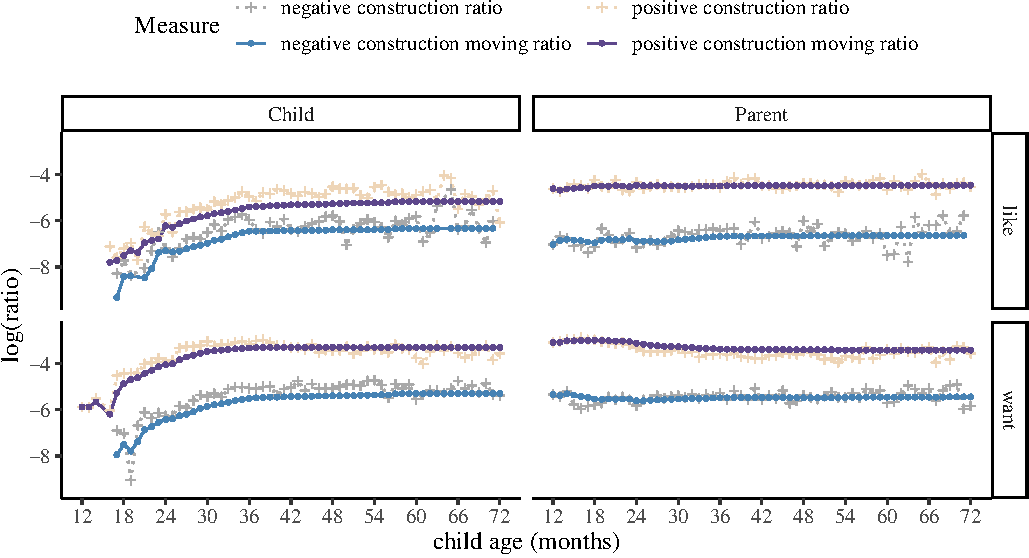
\includegraphics{neg_construction_article_files/figure-latex/emotion-1} 

}

\caption{Rejection and its positive counterparts}\label{fig:emotion}
\end{figure}

As presented in Figure 1, the overall pattern for children's usage of negative morphemes for rejection is comparable regardless of the particular head verb. Comparing child and parent speech, it seems that children's production of rejection is gradually increasing between the age of 18 to 36 months. And the production moving ratio in child speech appears to be more comparable to that of parent speech after 32-34 months.

\begin{figure}[H]

{\centering 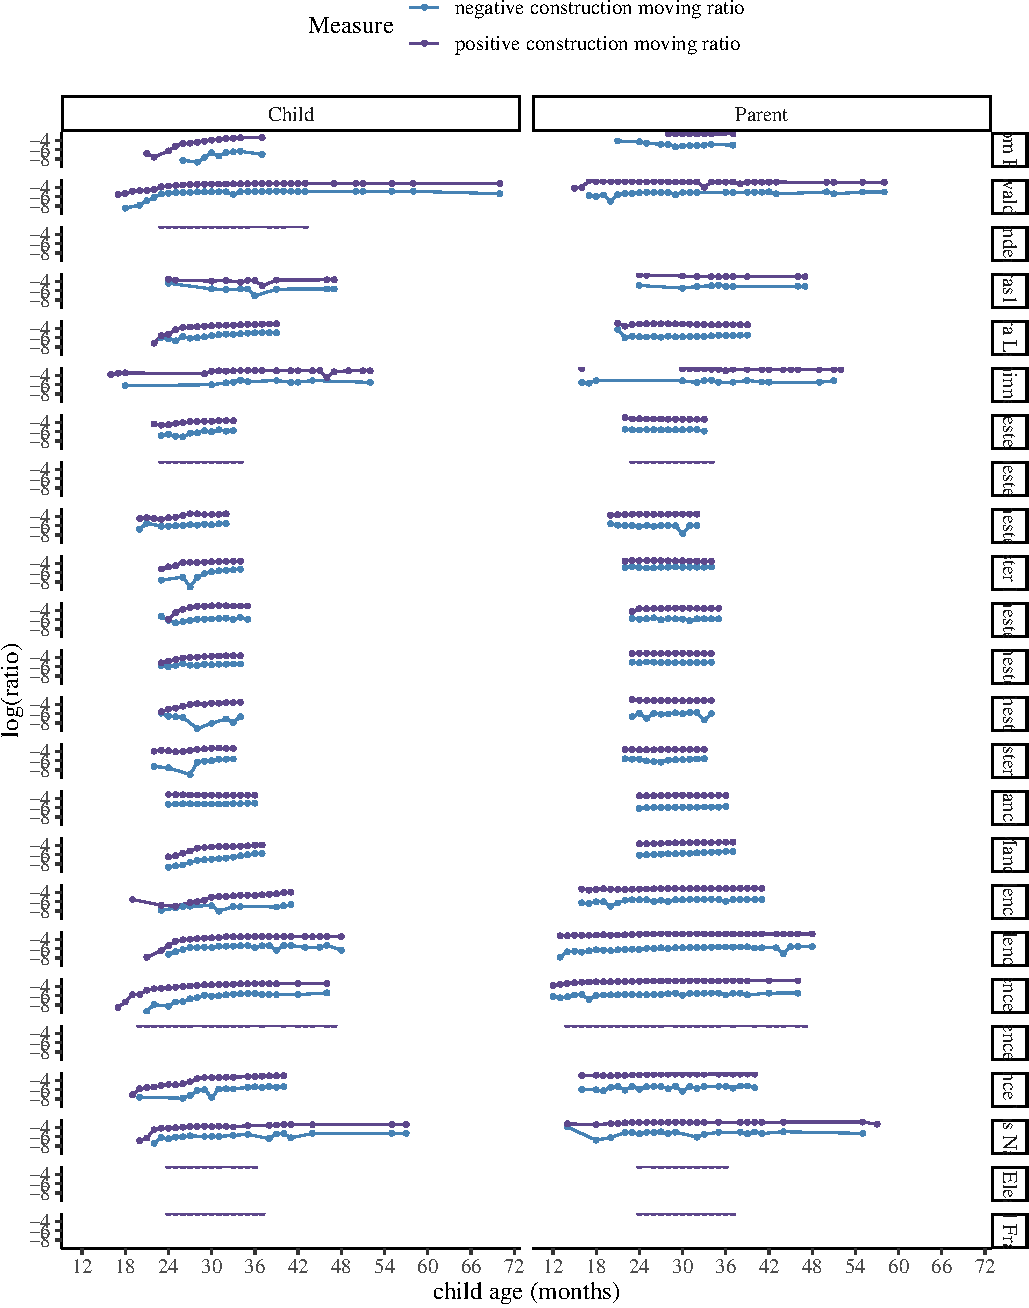
\includegraphics{neg_construction_article_files/figure-latex/individualemotion-1} 

}

\caption{Individual Variation for  Rejection and its positive counterparts}\label{fig:individualemotion}
\end{figure}

\begin{figure}[H]

{\centering 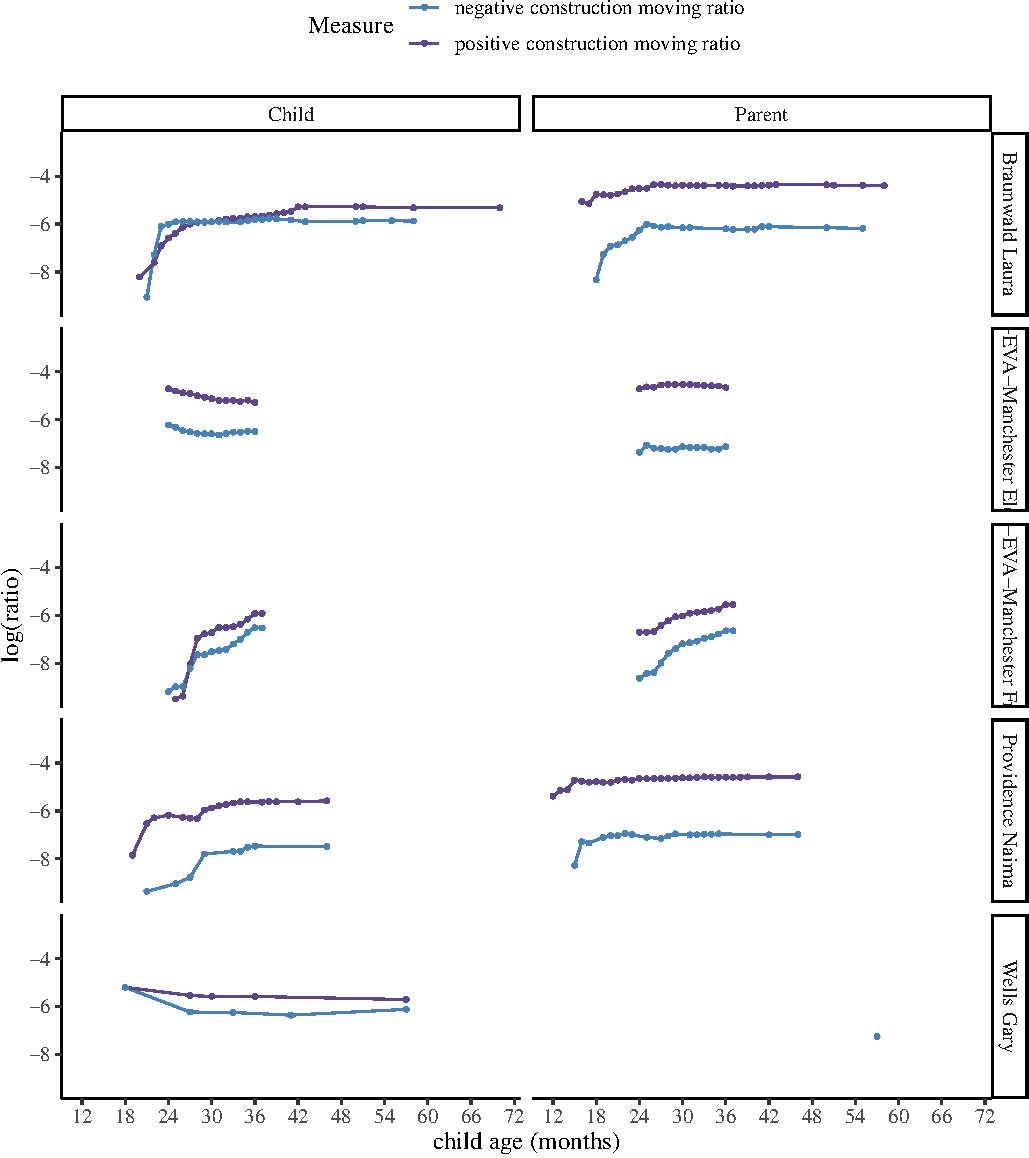
\includegraphics{neg_construction_article_files/figure-latex/individualemotionlike-1} 

}

\caption{Individual Variation for  Rejection and its positive counterparts, when the head verb is like}\label{fig:individualemotionlike}
\end{figure}

\begin{figure}[H]

{\centering 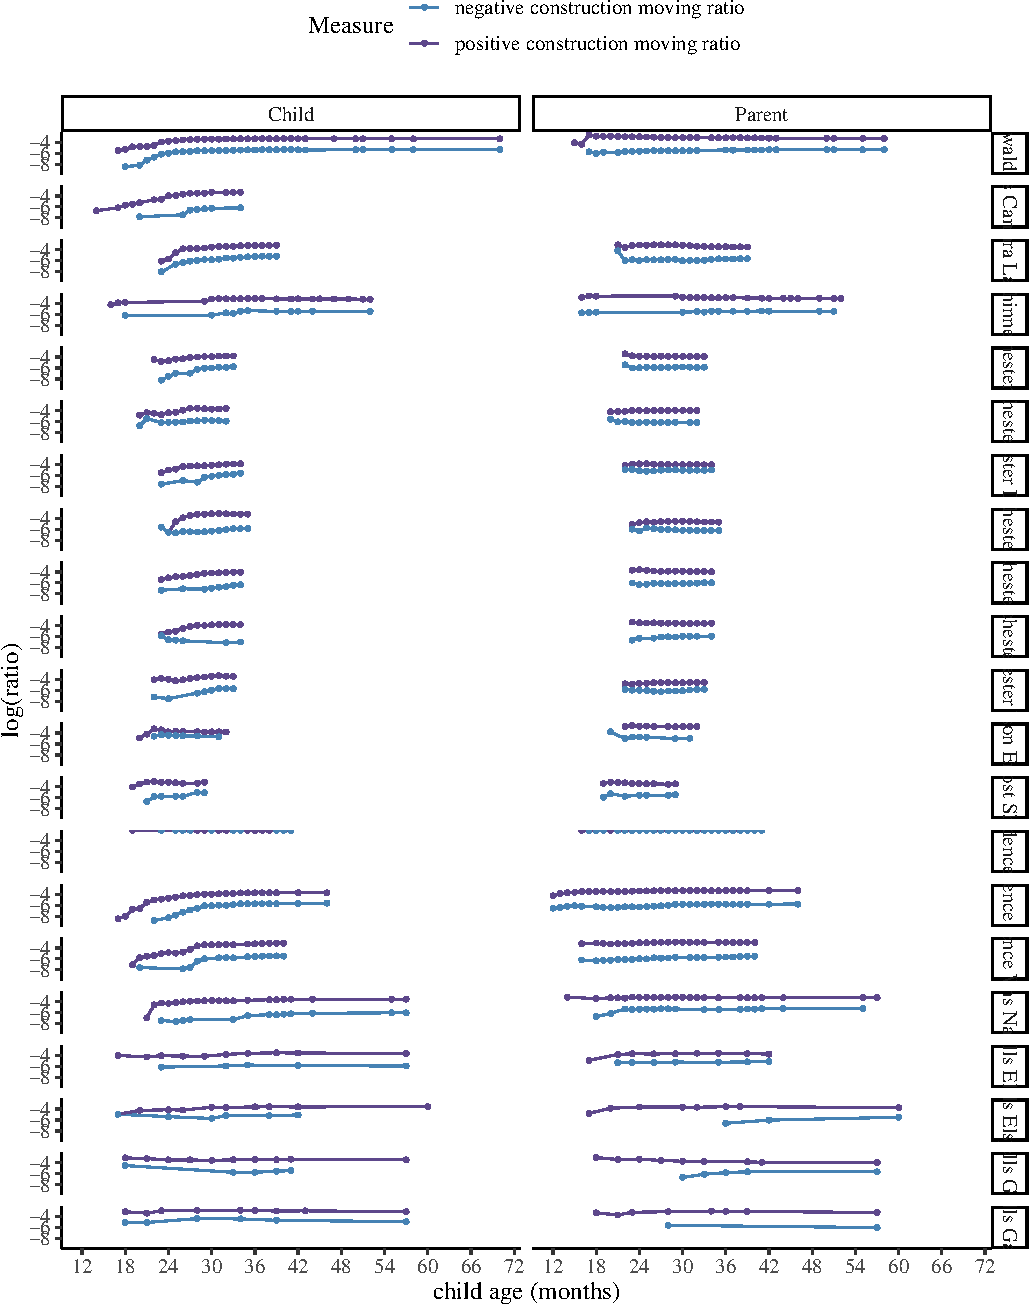
\includegraphics{neg_construction_article_files/figure-latex/individualemotionwant-1} 

}

\caption{Individual Variation for  Rejection and its positive counterparts, when the head verb is want}\label{fig:individualemotionwant}
\end{figure}

\clearpage

\hypertarget{non-existence}{%
\subsubsection{Non-existence}\label{non-existence}}

For the function of non-existence, we extracted utterances that have expletives marked by \emph{there} (e.g.~(5) and (6)), and that the predicate modified by the negative morphemes is a nominal phrase (headed by either nouns or pronouns). This led to a total of 30,609 negative utterances (child: 6,639; parent: 23,970).

~
(5) \emph{there's no (more) water}

~
(6) \emph{there isn't it}

In child speech, the production of negative constructions to express non-existence is gradually increasing from 25 to 36 months (Figure 2), which is by contrast later than that for the communicative function of rejection presented in Figure 1. This observation does not seem to align with Bloom (1970), which initially proposed that the development of non-existence is earlier than that of rejection. On the other hand, children's production moving ratio gradually approaches that in parent speech at 36-38 months.

Notice that there appears to be fluctuations of moving ratios between the age of 19 and 25 months regarding child production. A closer inspection of the data reveals that within that age range, the frequency of negative utterances at most ages is either one or zero. Therefore while the number of total utterances increases along the developmental trajectory, the moving ratio for negative utterances actually decreases.

\begin{figure}[H]

{\centering 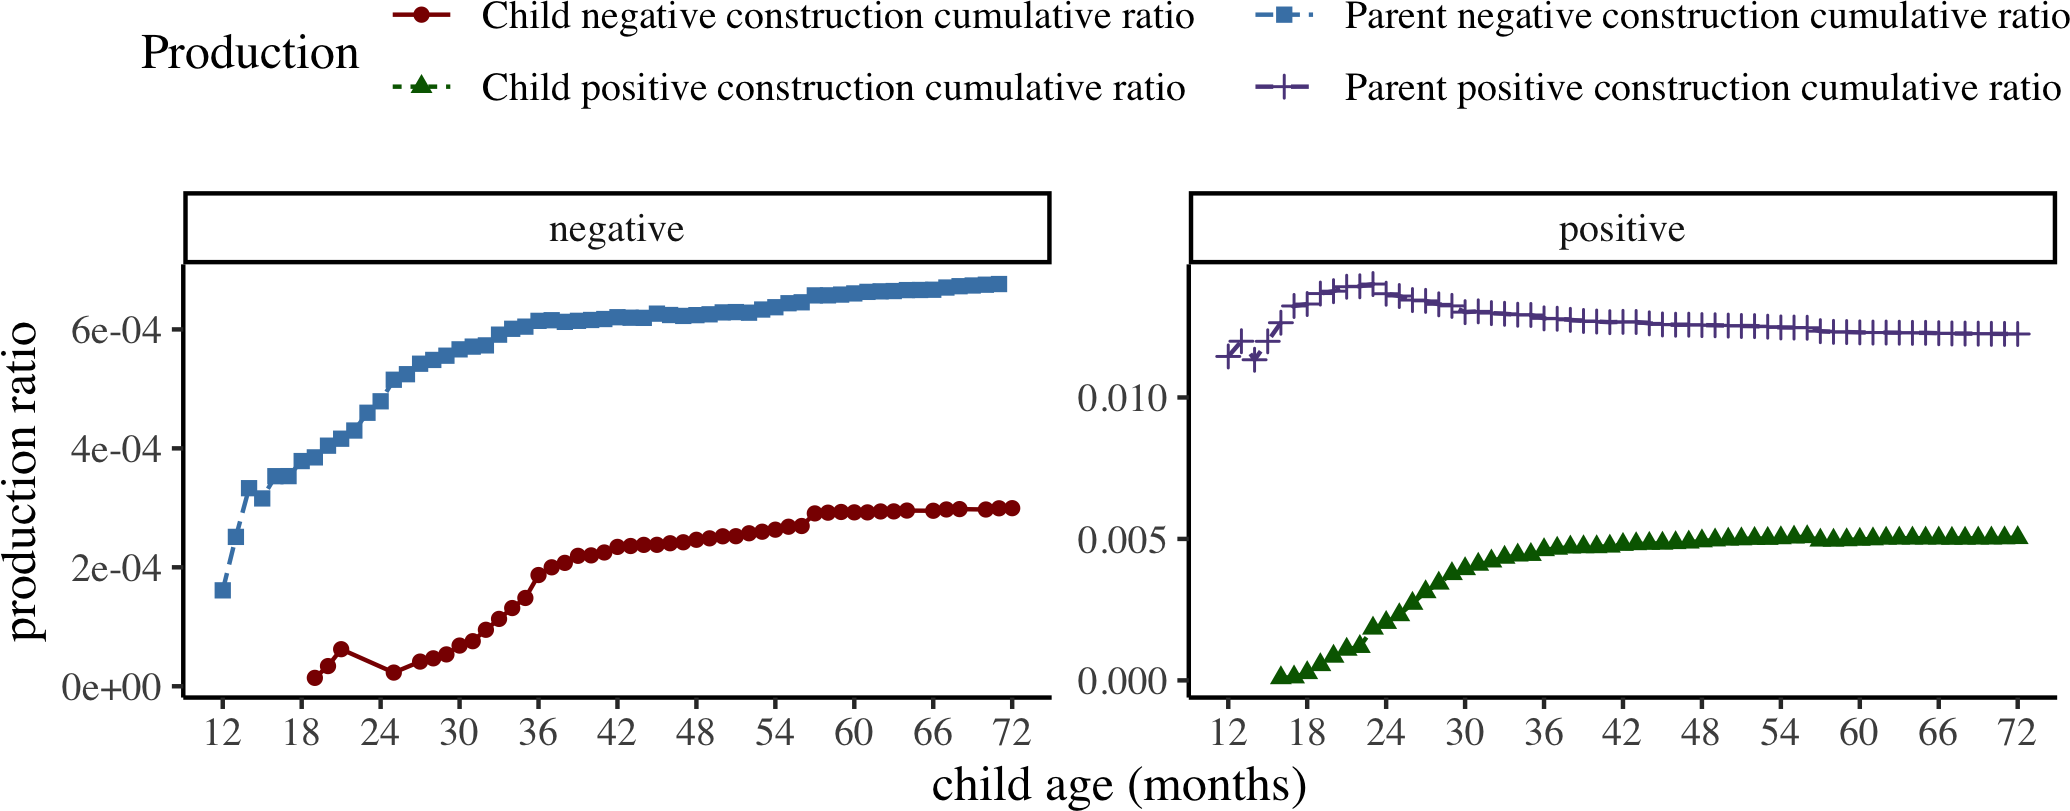
\includegraphics{neg_construction_article_files/figure-latex/existence-1} 

}

\caption{Non-existence and its positive counterparts}\label{fig:existence}
\end{figure}

\begin{figure}[H]

{\centering 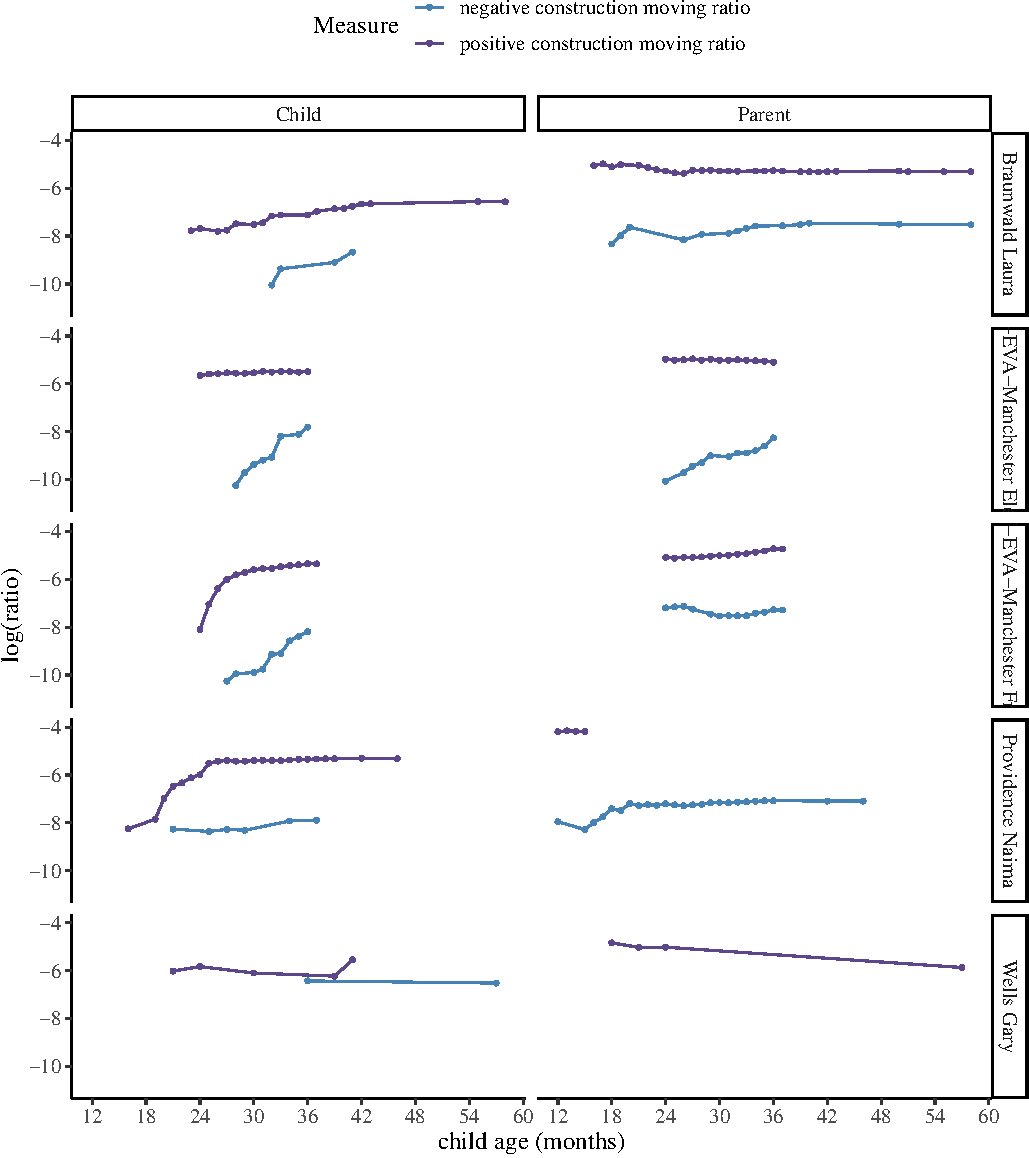
\includegraphics{neg_construction_article_files/figure-latex/individualexistence-1} 

}

\caption{Individual variation for Non-existence and its positive counterparts}\label{fig:individualexistence}
\end{figure}

\hypertarget{prohibition}{%
\subsubsection{Prohibition}\label{prohibition}}

For constructions that articulate the function of prohibition, we focused on cases that are annotated as imperatives from the initial CHILDES annotations. These utterances do not take any subject; the negative morphemes are combined with the auxiliary verb \emph{do} (\emph{do}, \emph{does}, \emph{did}) and they together modify the head verbs of the sentences.
In order to not overlap with rejection, non-existence, epistemic negation and possession (see below), our search excluded cases where the head verb has any of the following lemma forms: \emph{like}, \emph{want}, \emph{know}, \emph{think}, \emph{remember}, \emph{have}. This resulted in a total of 18,586 negative utterances (child: 6,431; parent: 12,155).

Based on Figure 3, children are combining negative morphemes for prohibition more and more regularly between 24-36 months, which is comparable to that of the function of non-existence, but slightly later than that of rejection. In comparison, the production moving ratio in child speech for prohibition is consistently lower than that in parent speech at any age of the children.

~
(7) \emph{don't blame Charlotte}

\begin{figure}[H]

{\centering 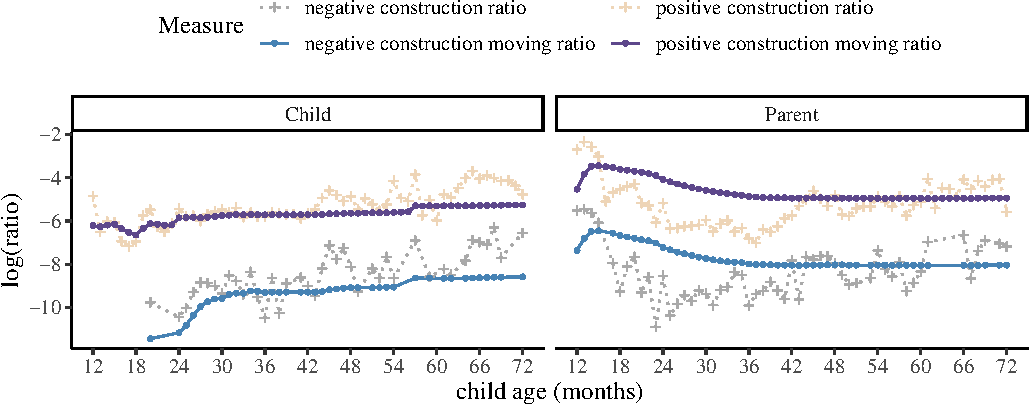
\includegraphics{neg_construction_article_files/figure-latex/prohibition-1} 

}

\caption{Prohibition and its positive counterparts}\label{fig:prohibition}
\end{figure}

\begin{figure}[H]

{\centering 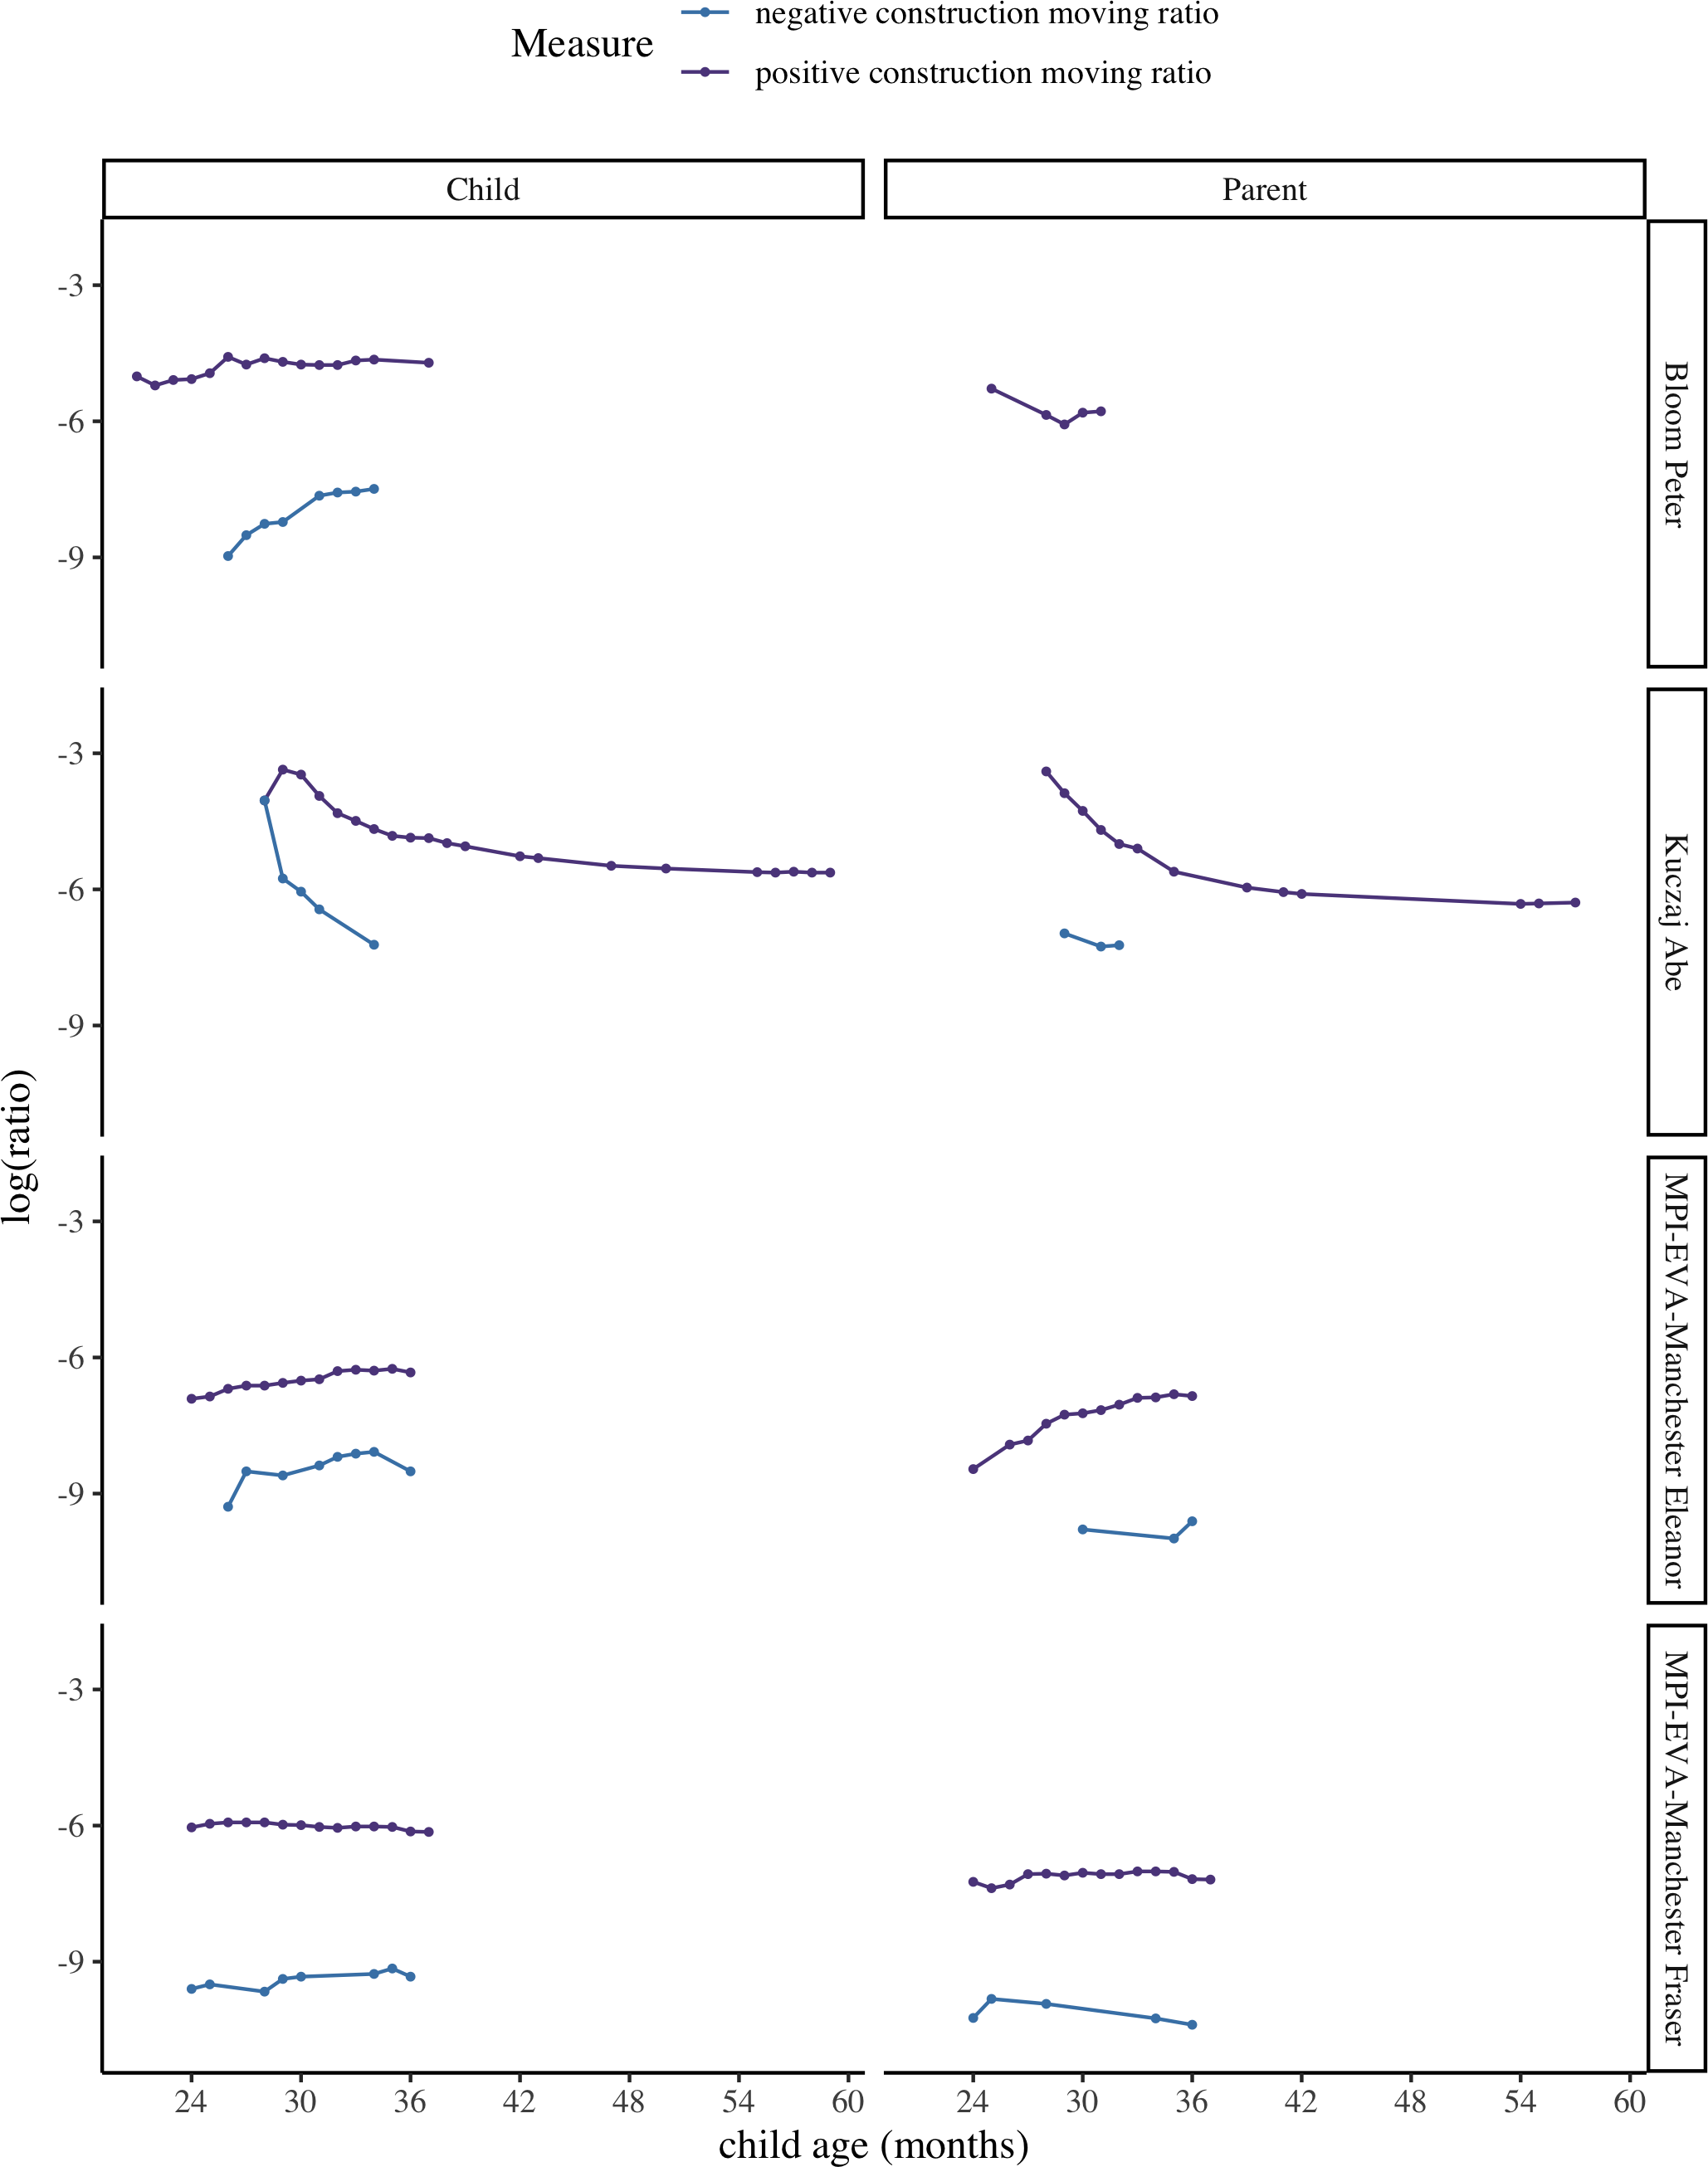
\includegraphics{neg_construction_article_files/figure-latex/individualprohibition-1} 

}

\caption{Individual variation for Prohibition and its positive counterparts}\label{fig:individualprohibition}
\end{figure}

\clearpage

\hypertarget{inability}{%
\subsubsection{Inability}\label{inability}}

For the function of inability, we analyzed instances where the negative morphemes co-occur with the auxiliary \emph{can} (\emph{can} and \emph{could}; e.g.~(8)) and both of them modify the head verbs of the utterances. Again, we filtered out cases where the head verbs are the focus for other functions. Cases without a subject (e.g.~\enquote{can't play}) or where the subject is not \emph{I} (e.g.~\enquote{you can't do that}) could yield ambiguous readings when not looking at a larger discourse context; they could be a rhetorical question or also express the concept of prohibition. Therefore to potentially avoid less ambiguity, we restricted our analyses only to cases with a subject \emph{I}. This led to 110,879 negative utterances (child: 61,300; parent: 49,579).

~
(8) \emph{I can't see}

As shown in Figure 4, the developmental trajectory of inability is similar to that of rejection. Negation is applied more and more regularly between 18-36 months. By contrast, it is different from those of non-existence and prohibition. It seems that the production trajectories of the latter two are both becoming more regular at a later age (25 and 24 months, respectively).

\begin{figure}[H]

{\centering 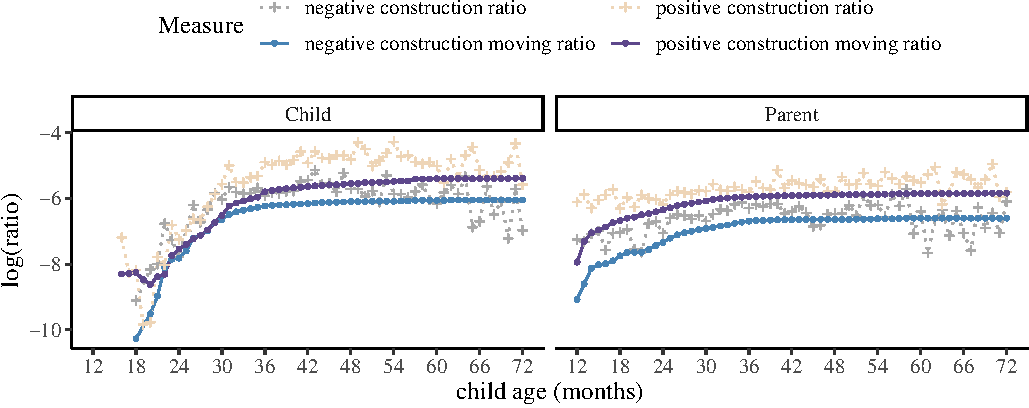
\includegraphics{neg_construction_article_files/figure-latex/inability-1} 

}

\caption{Inability and its positive counterparts}\label{fig:inability}
\end{figure}

\begin{figure}[H]

{\centering 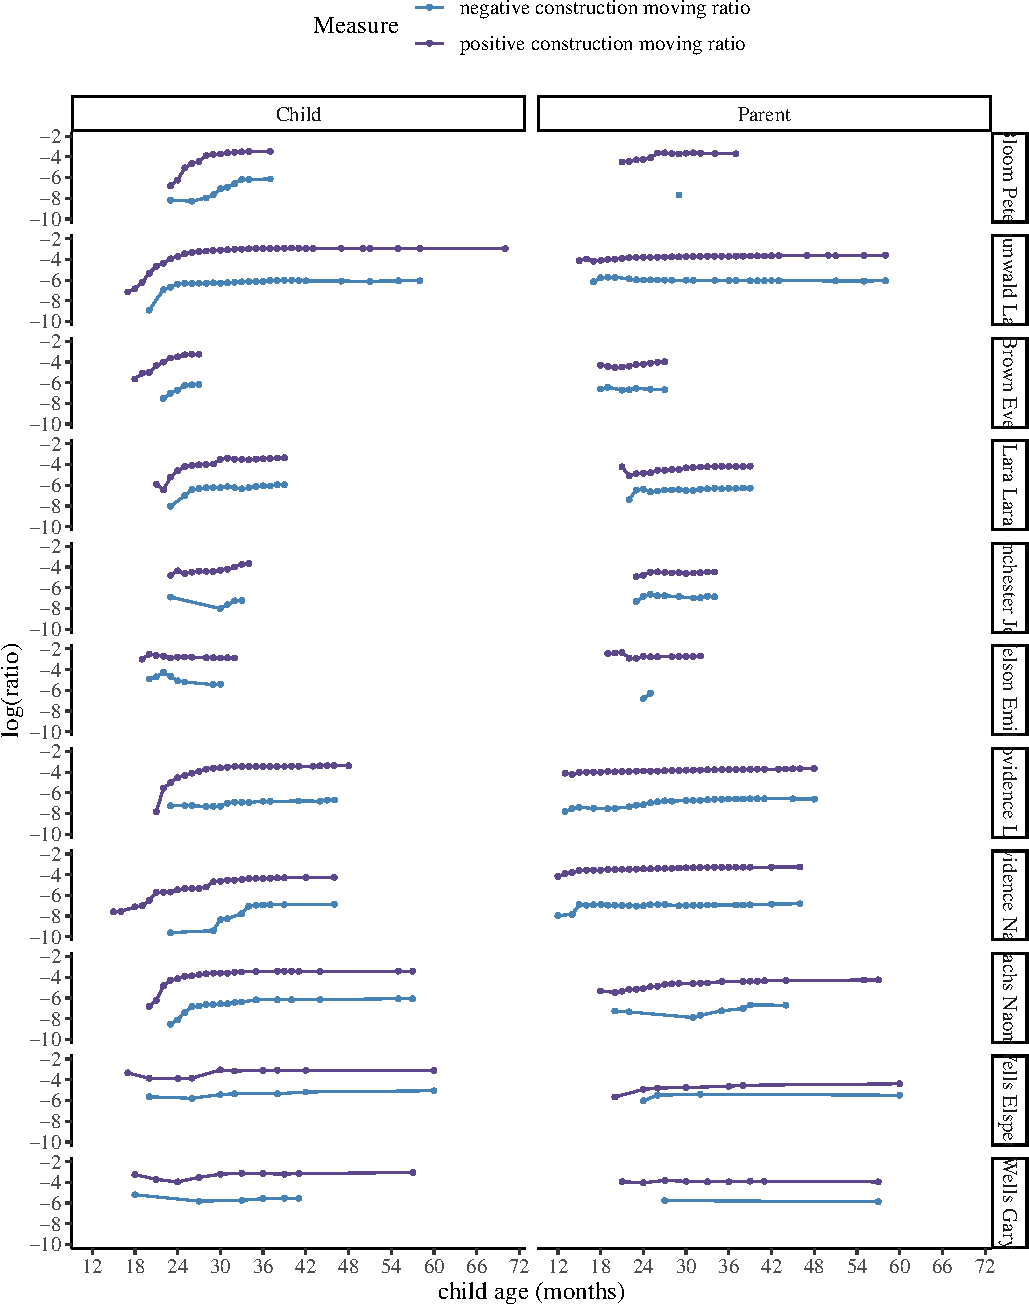
\includegraphics{neg_construction_article_files/figure-latex/individualinability-1} 

}

\caption{Individual variation for Inability and its positive counterparts}\label{fig:individualinability}
\end{figure}

\clearpage

\hypertarget{labeling}{%
\subsubsection{Labeling}\label{labeling}}

To capture the function of labeling, we concentrated on cases where negative morphemes indicate the identity (e.g.~(9)), and/or characteristics (e.g.~(10)) of a predicative nominal. We also included instances where negation is used to modify a predicative adjective (e.g.~(11)). Utterances where negative morphemes modify a nominal or adjectival predicate of a copula verb were extracted. None of the utterances contained expletives (e.g.~\enquote{there is no book}) to distinguish from non-existence. This resulted in a total of 377,128 negative utterances (Child: 88,552; Parent: 288,576).

~
(9) \emph{that's not a farmer}

~
(10) \emph{I'm not a heavy baby Mum}

~
(11) \emph{It's no good}

Based on Figure 5, the developmental pattern for labeling is comparable to non-existence and prohibition; children are increasing their use of the negative morphemes around the age range of of 22-36 months.

\begin{figure}[H]

{\centering 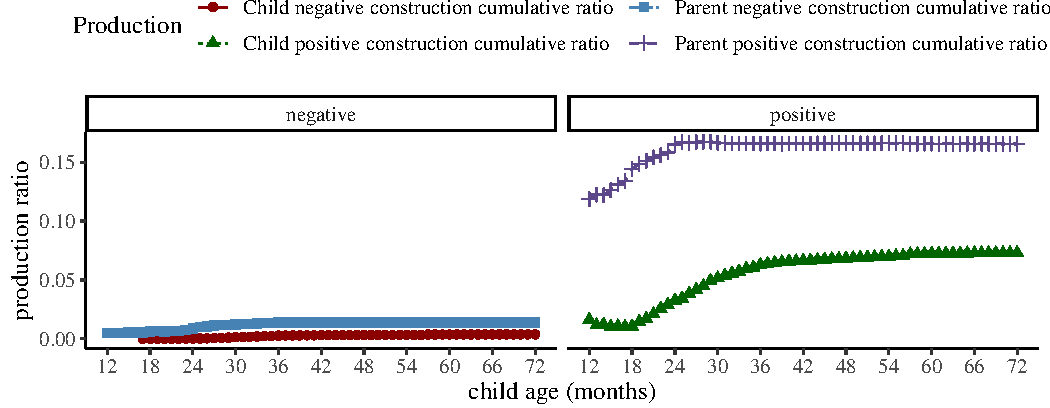
\includegraphics{neg_construction_article_files/figure-latex/learning-1} 

}

\caption{Labeling and its positive counterparts}\label{fig:learning}
\end{figure}

\begin{figure}[H]

{\centering 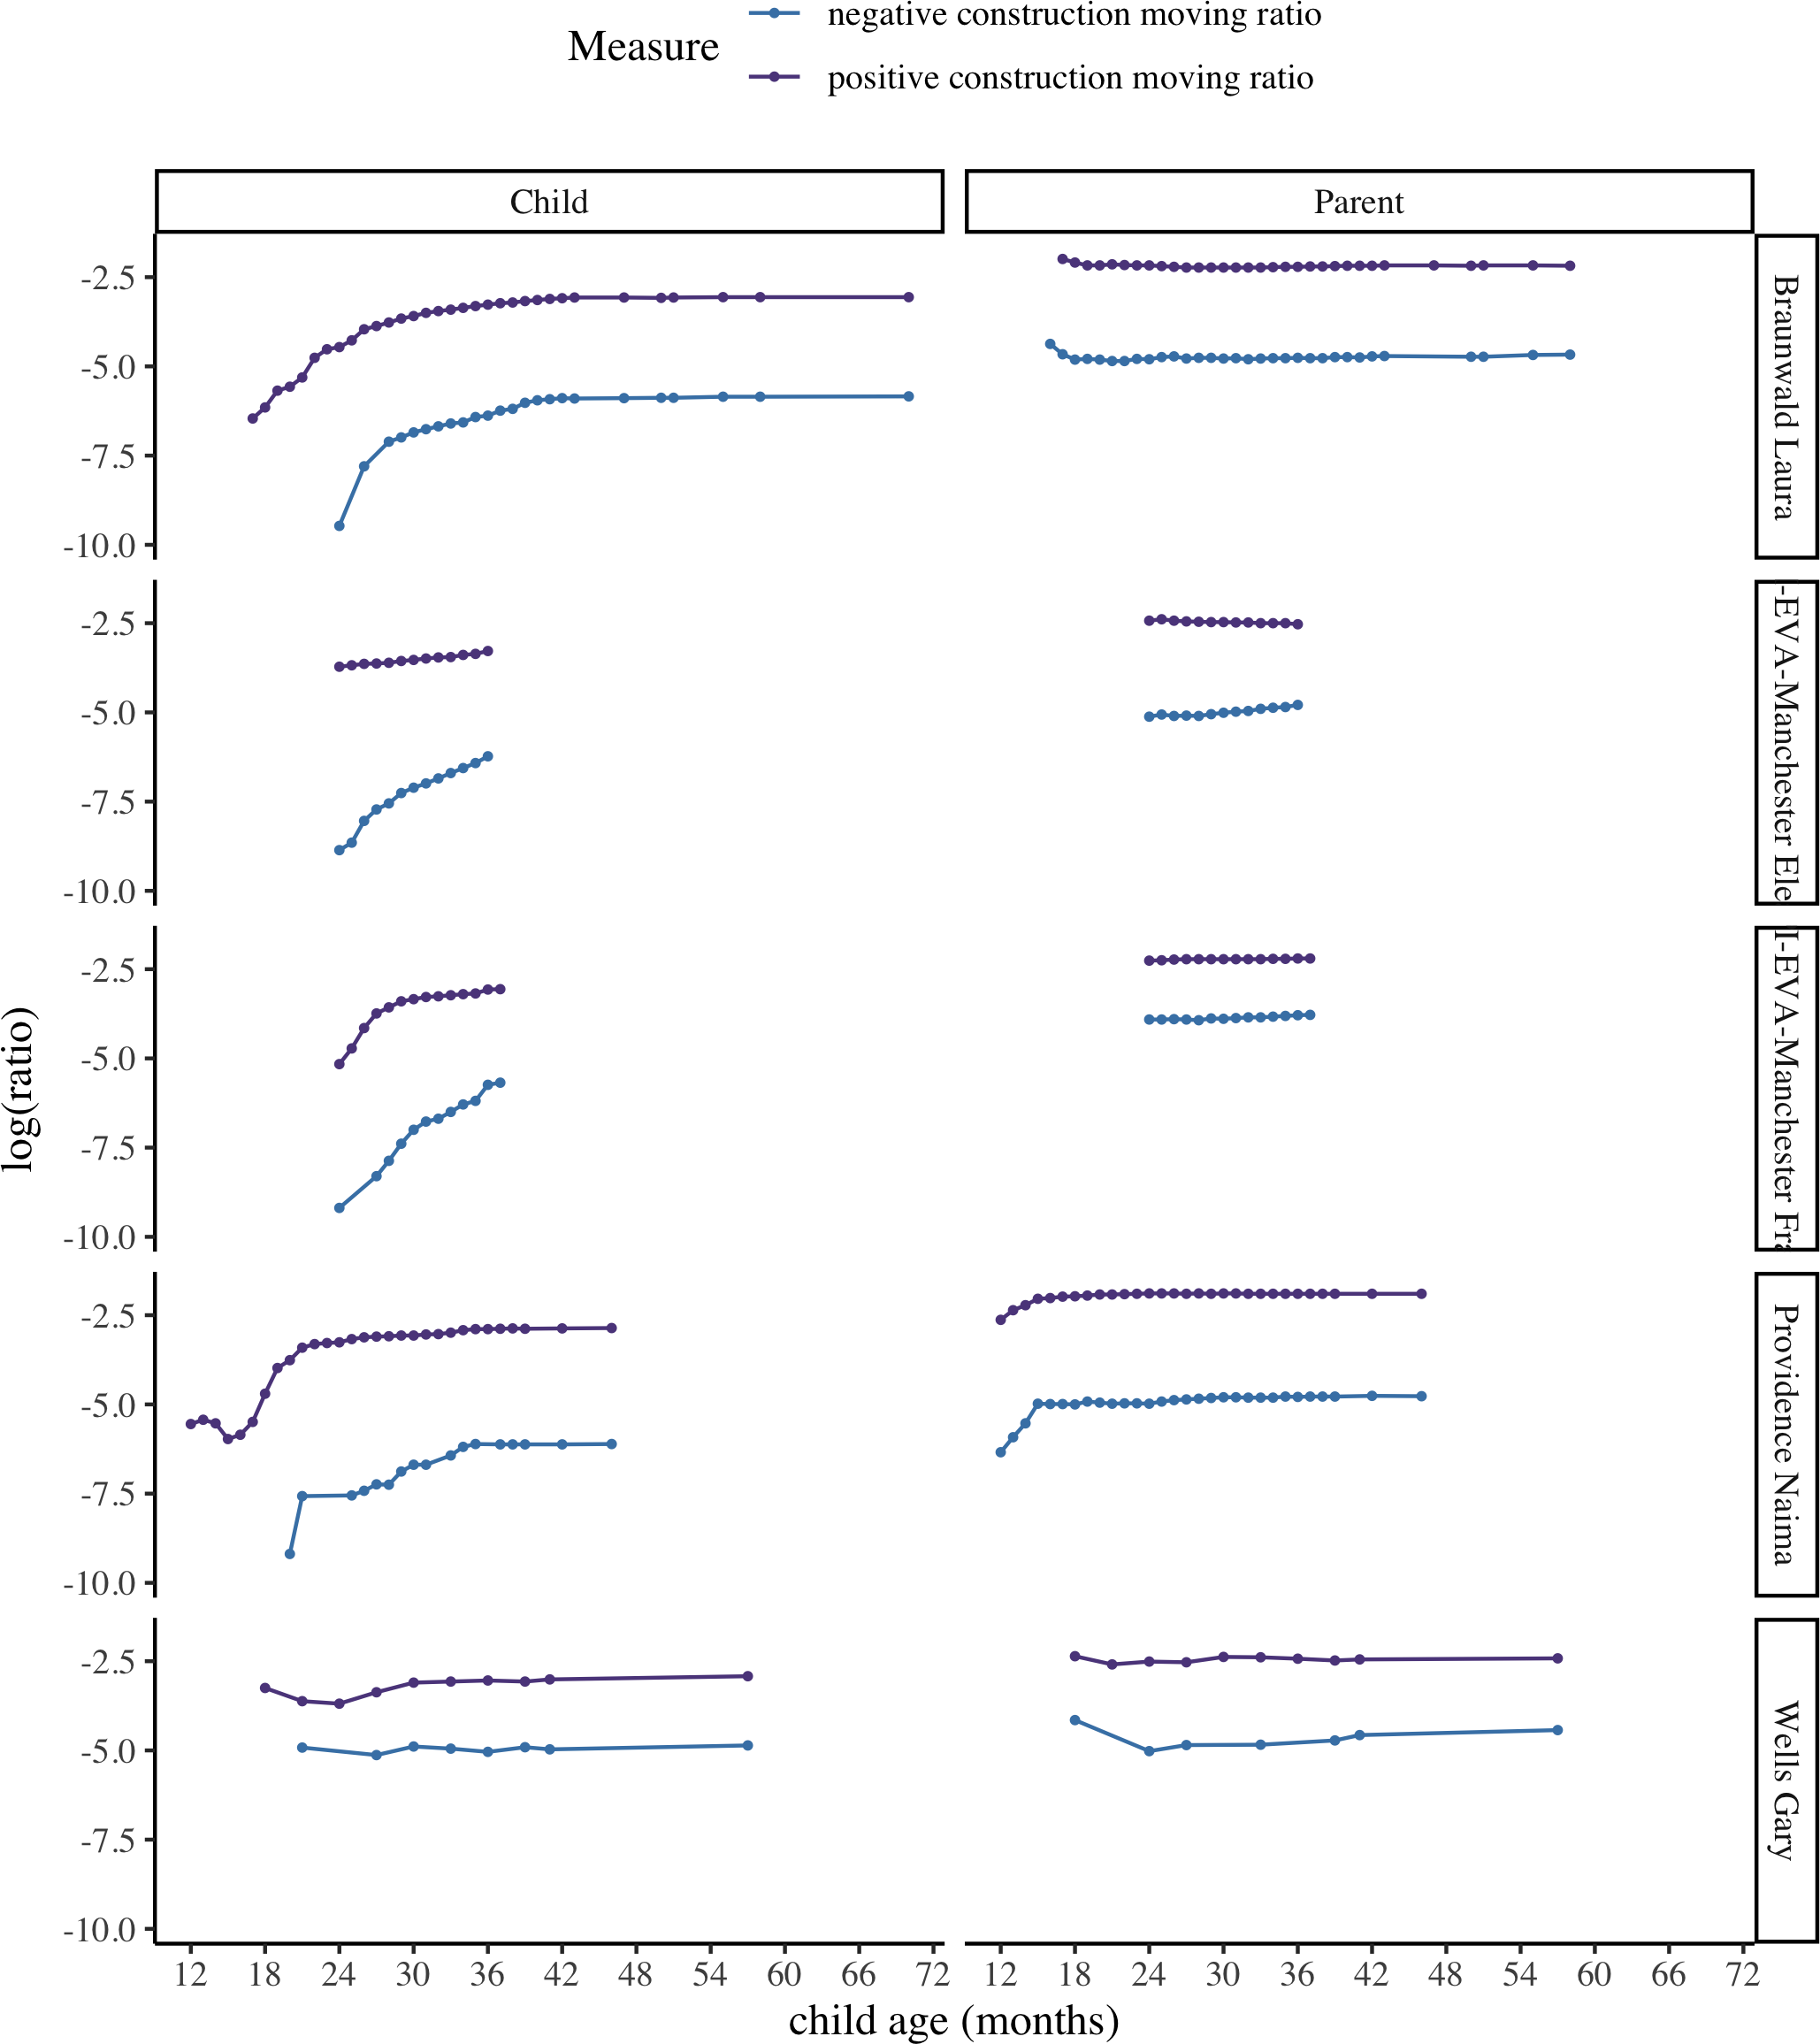
\includegraphics{neg_construction_article_files/figure-latex/individuallearning-1} 

}

\caption{Individual variation for Labeling and its positive counterparts}\label{fig:individuallearning}
\end{figure}

\clearpage

\hypertarget{epistemic-negation}{%
\subsubsection{Epistemic Negation}\label{epistemic-negation}}

Previous studies have reported instances where negative morphemes are combined with mental/epistemic state verbs such as \emph{know}, \emph{think}, and \emph{remember} in child speech to express epistemic negation. Here we focused on these three verbs and analyzed negative utterances that articulate the concept of not knowing (e.g.~(12)) or uncertainty (e.g.~(13)). The verbs in these cases are modified by the negative morphemes directly or by the combination of negation with auxiliaries. Instances where the speaker asks about or describes the negative epistemic state of another speaker (e.g.~(14)) were also selected, leading to 109,325 negative utterances in total (child: 18,581; parent: 90,744).

~
(12) \emph{I not know} / \emph{I didn't remember}

~
(13) \emph{I don't think so}

~
(14) \emph{don't you remember} / \emph{She doesn't know this}

Based on the data analyzed here (Figure 6), the production of negative utterances headed by \emph{know} are becoming more regular at an earlier age (17-18 months) compared to that of \emph{remember} (\textasciitilde19 months) or \emph{think} (\textasciitilde20 months). Overall the production moving ratio of utterances with \emph{know} is comparatively the highest.

\begin{figure}[H]

{\centering 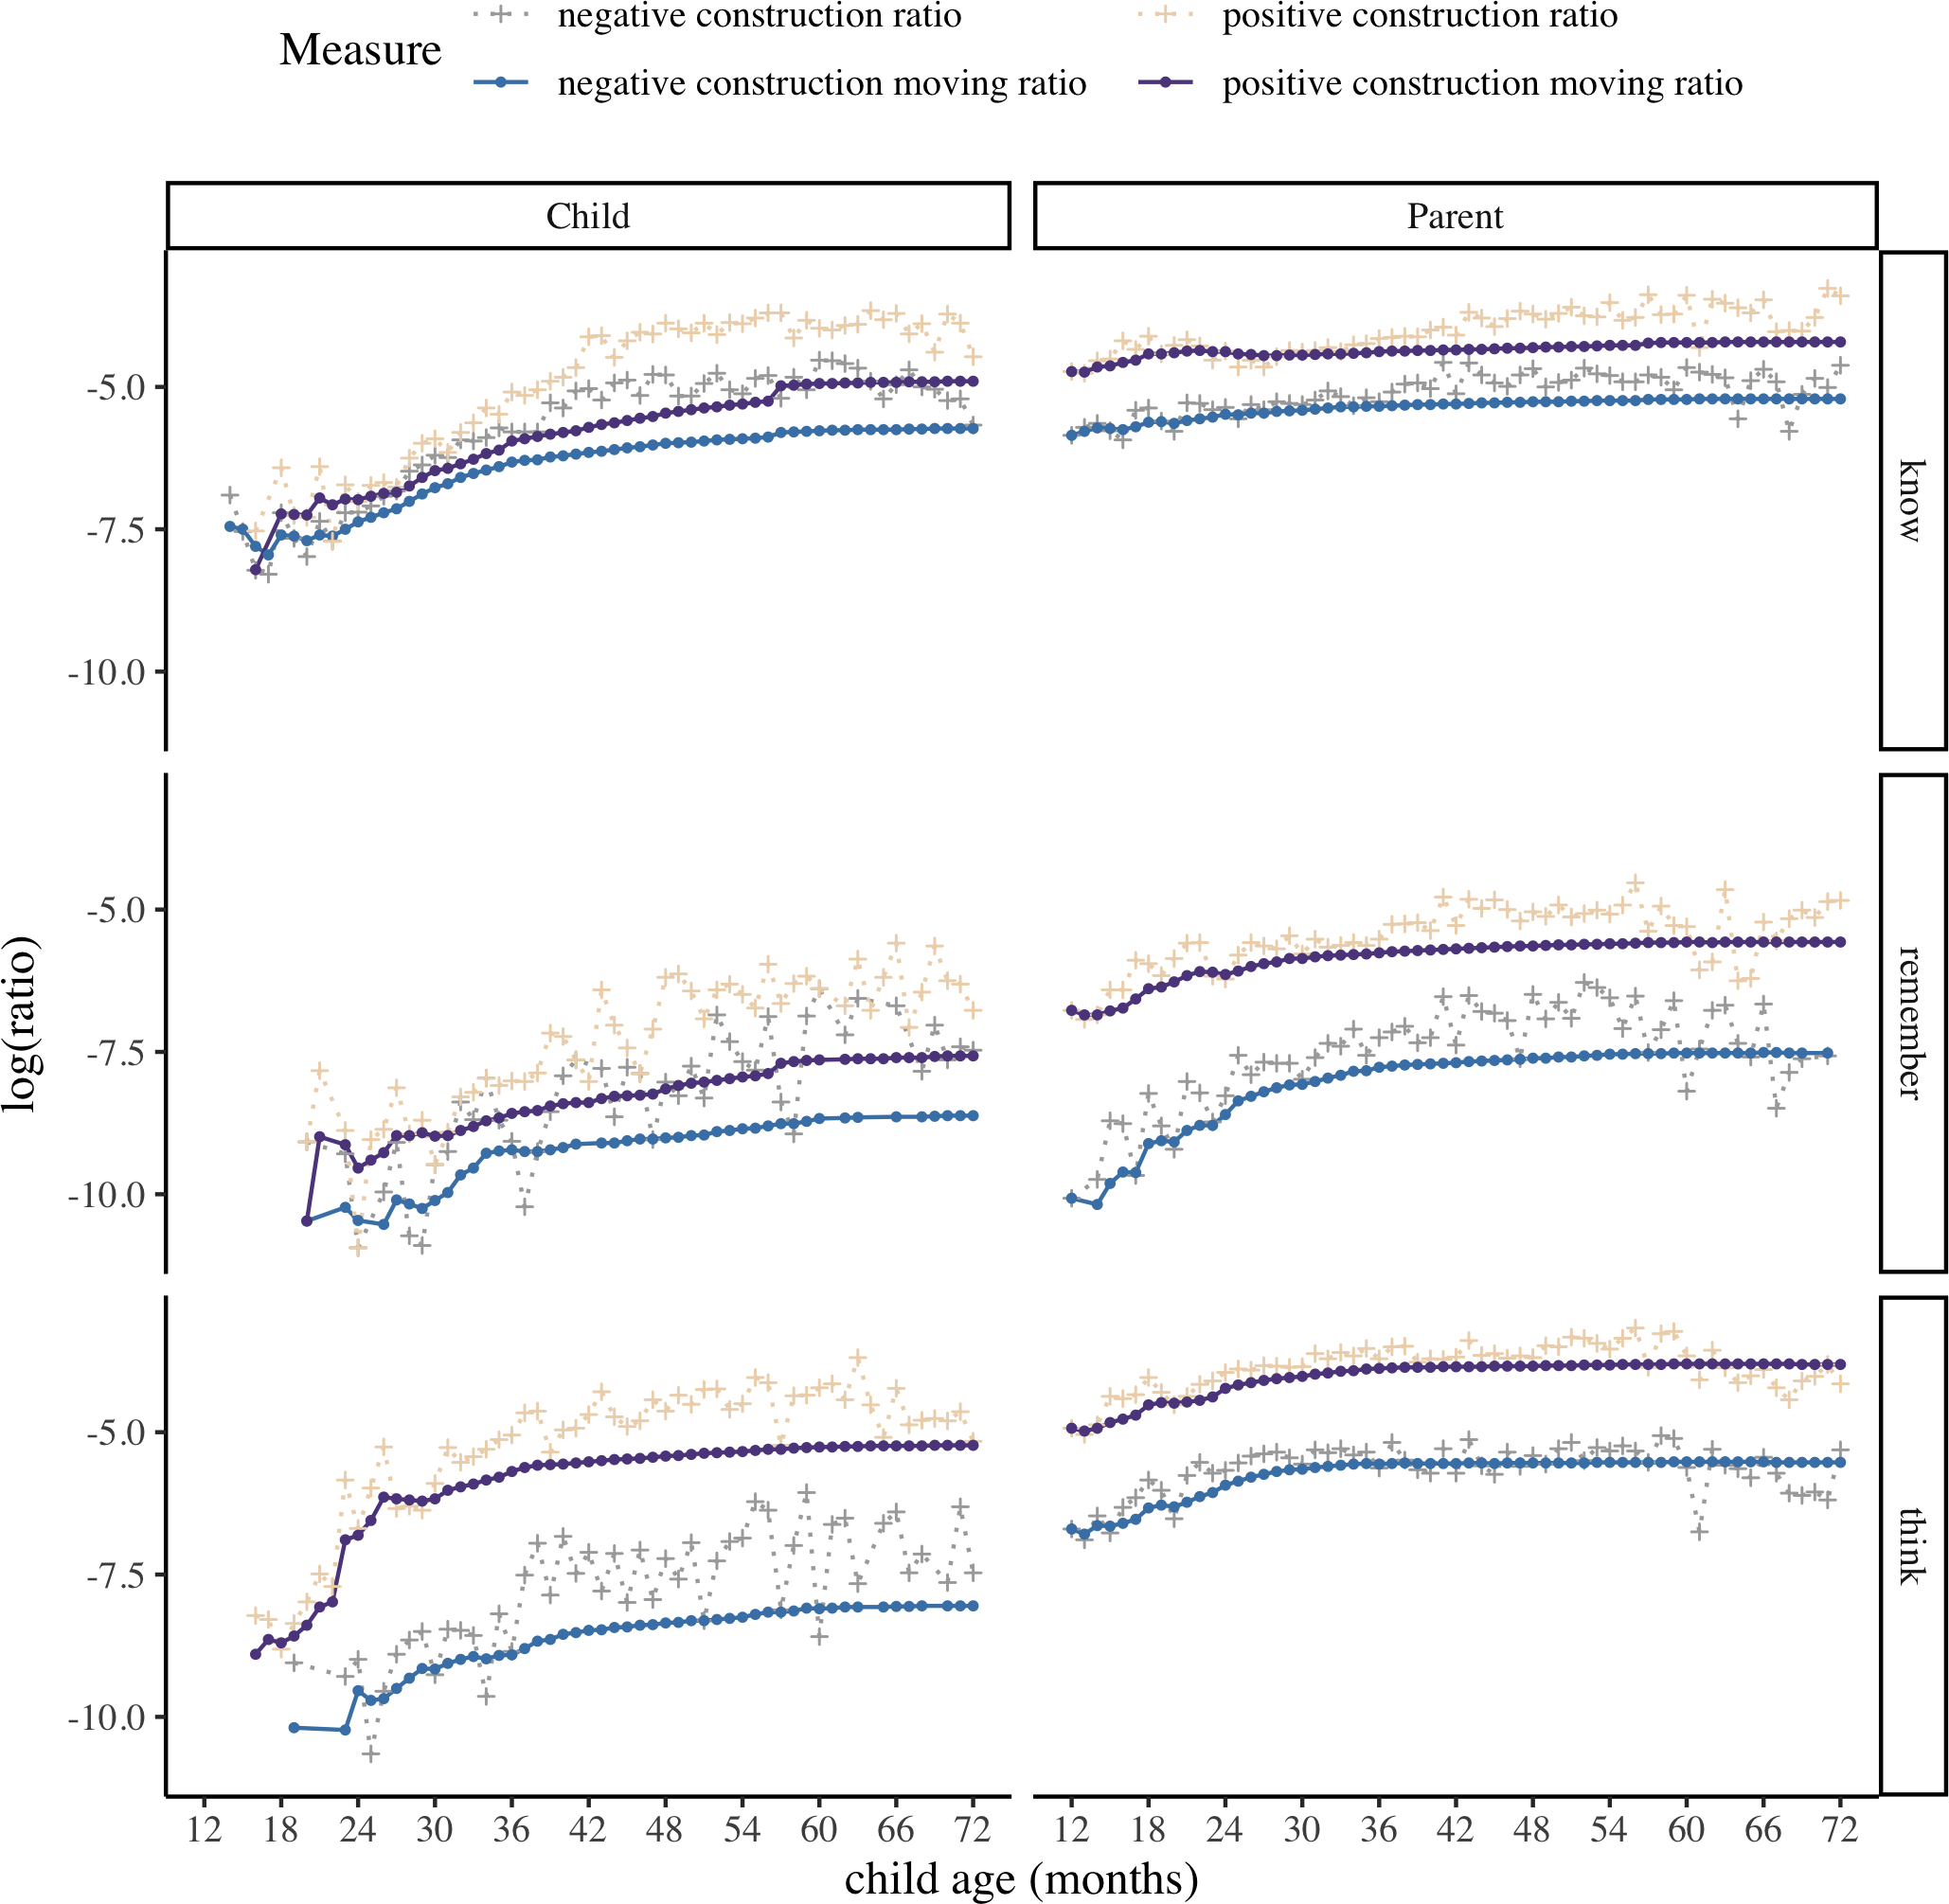
\includegraphics{neg_construction_article_files/figure-latex/epistemic-1} 

}

\caption{Epistemic negation and its positive counterparts}\label{fig:epistemic}
\end{figure}

\begin{figure}[H]

{\centering 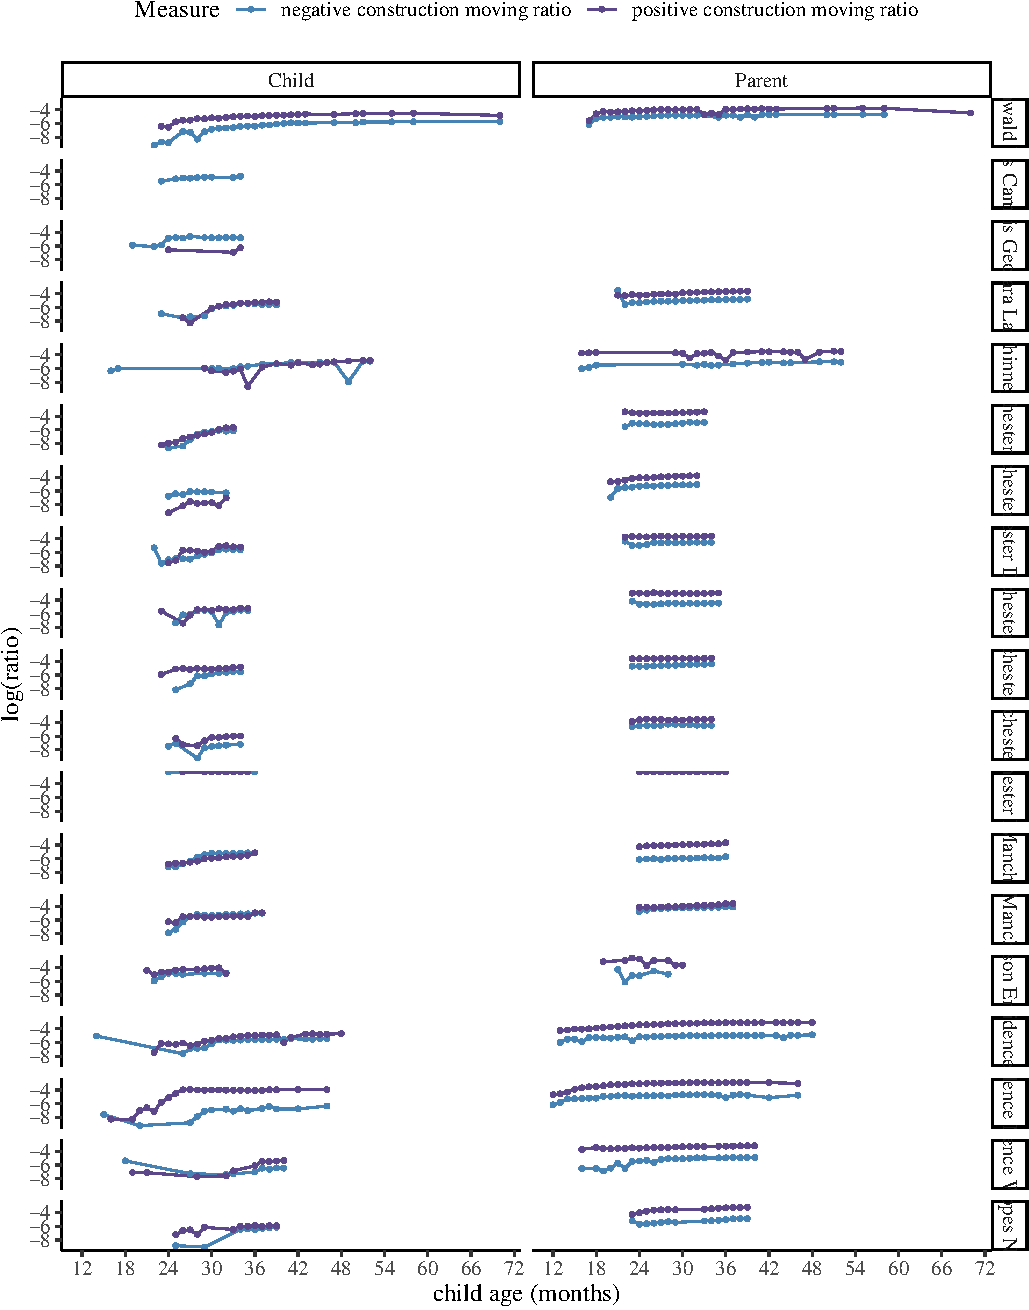
\includegraphics{neg_construction_article_files/figure-latex/individualepistemic-1} 

}

\caption{Individual variation for Epistemic negation and its positive counterparts}\label{fig:individualepistemic}
\end{figure}

\begin{figure}[H]

{\centering 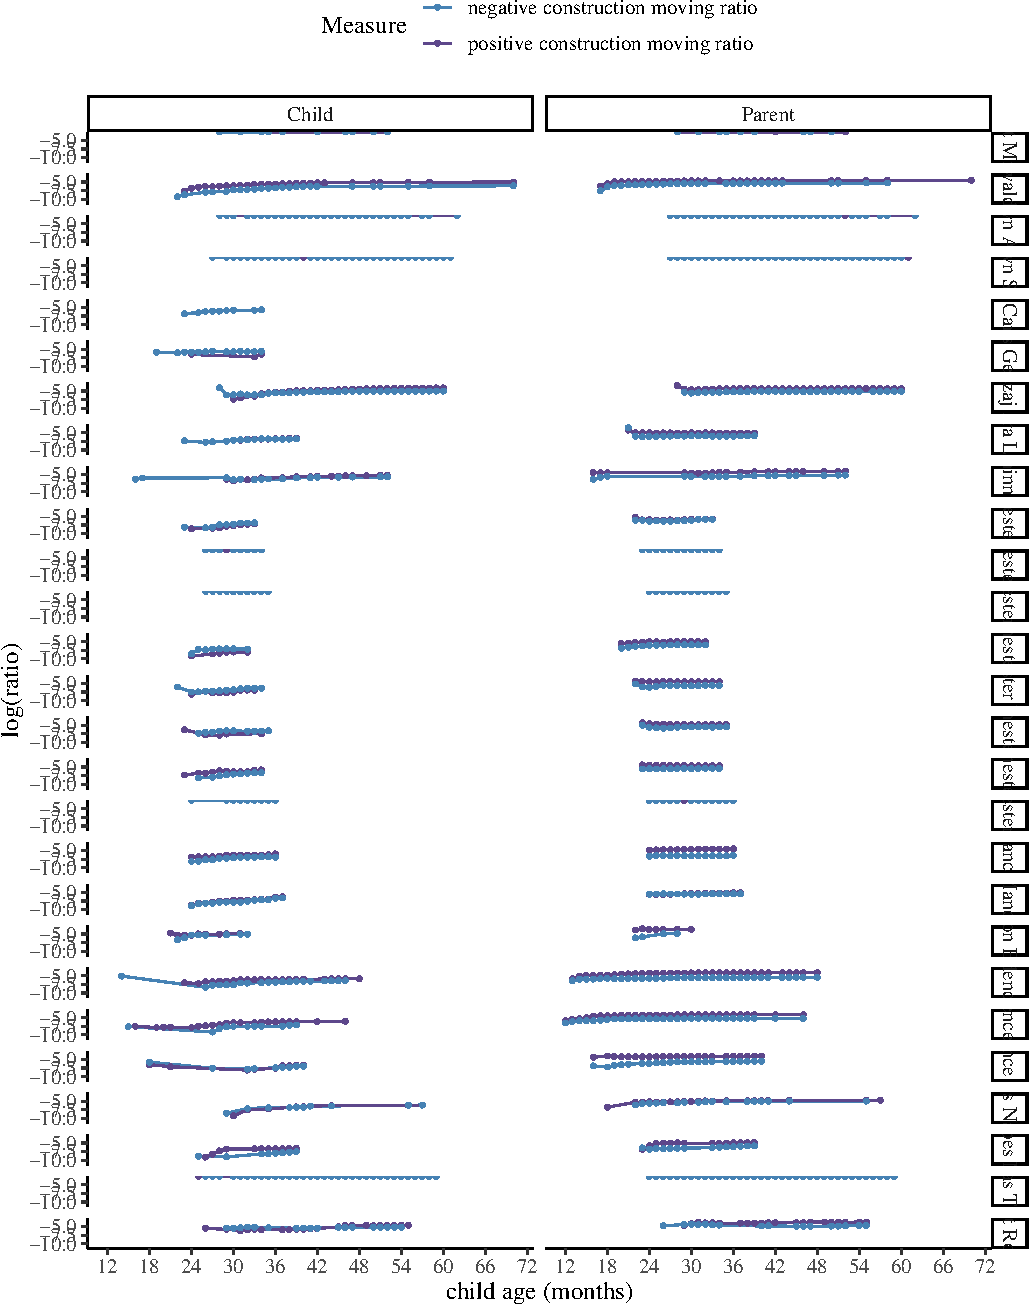
\includegraphics{neg_construction_article_files/figure-latex/individualepistemicknow-1} 

}

\caption{Individual variation for Epistemic negation and its positive counterparts, when the head verb is know}\label{fig:individualepistemicknow}
\end{figure}

\begin{figure}[H]

{\centering 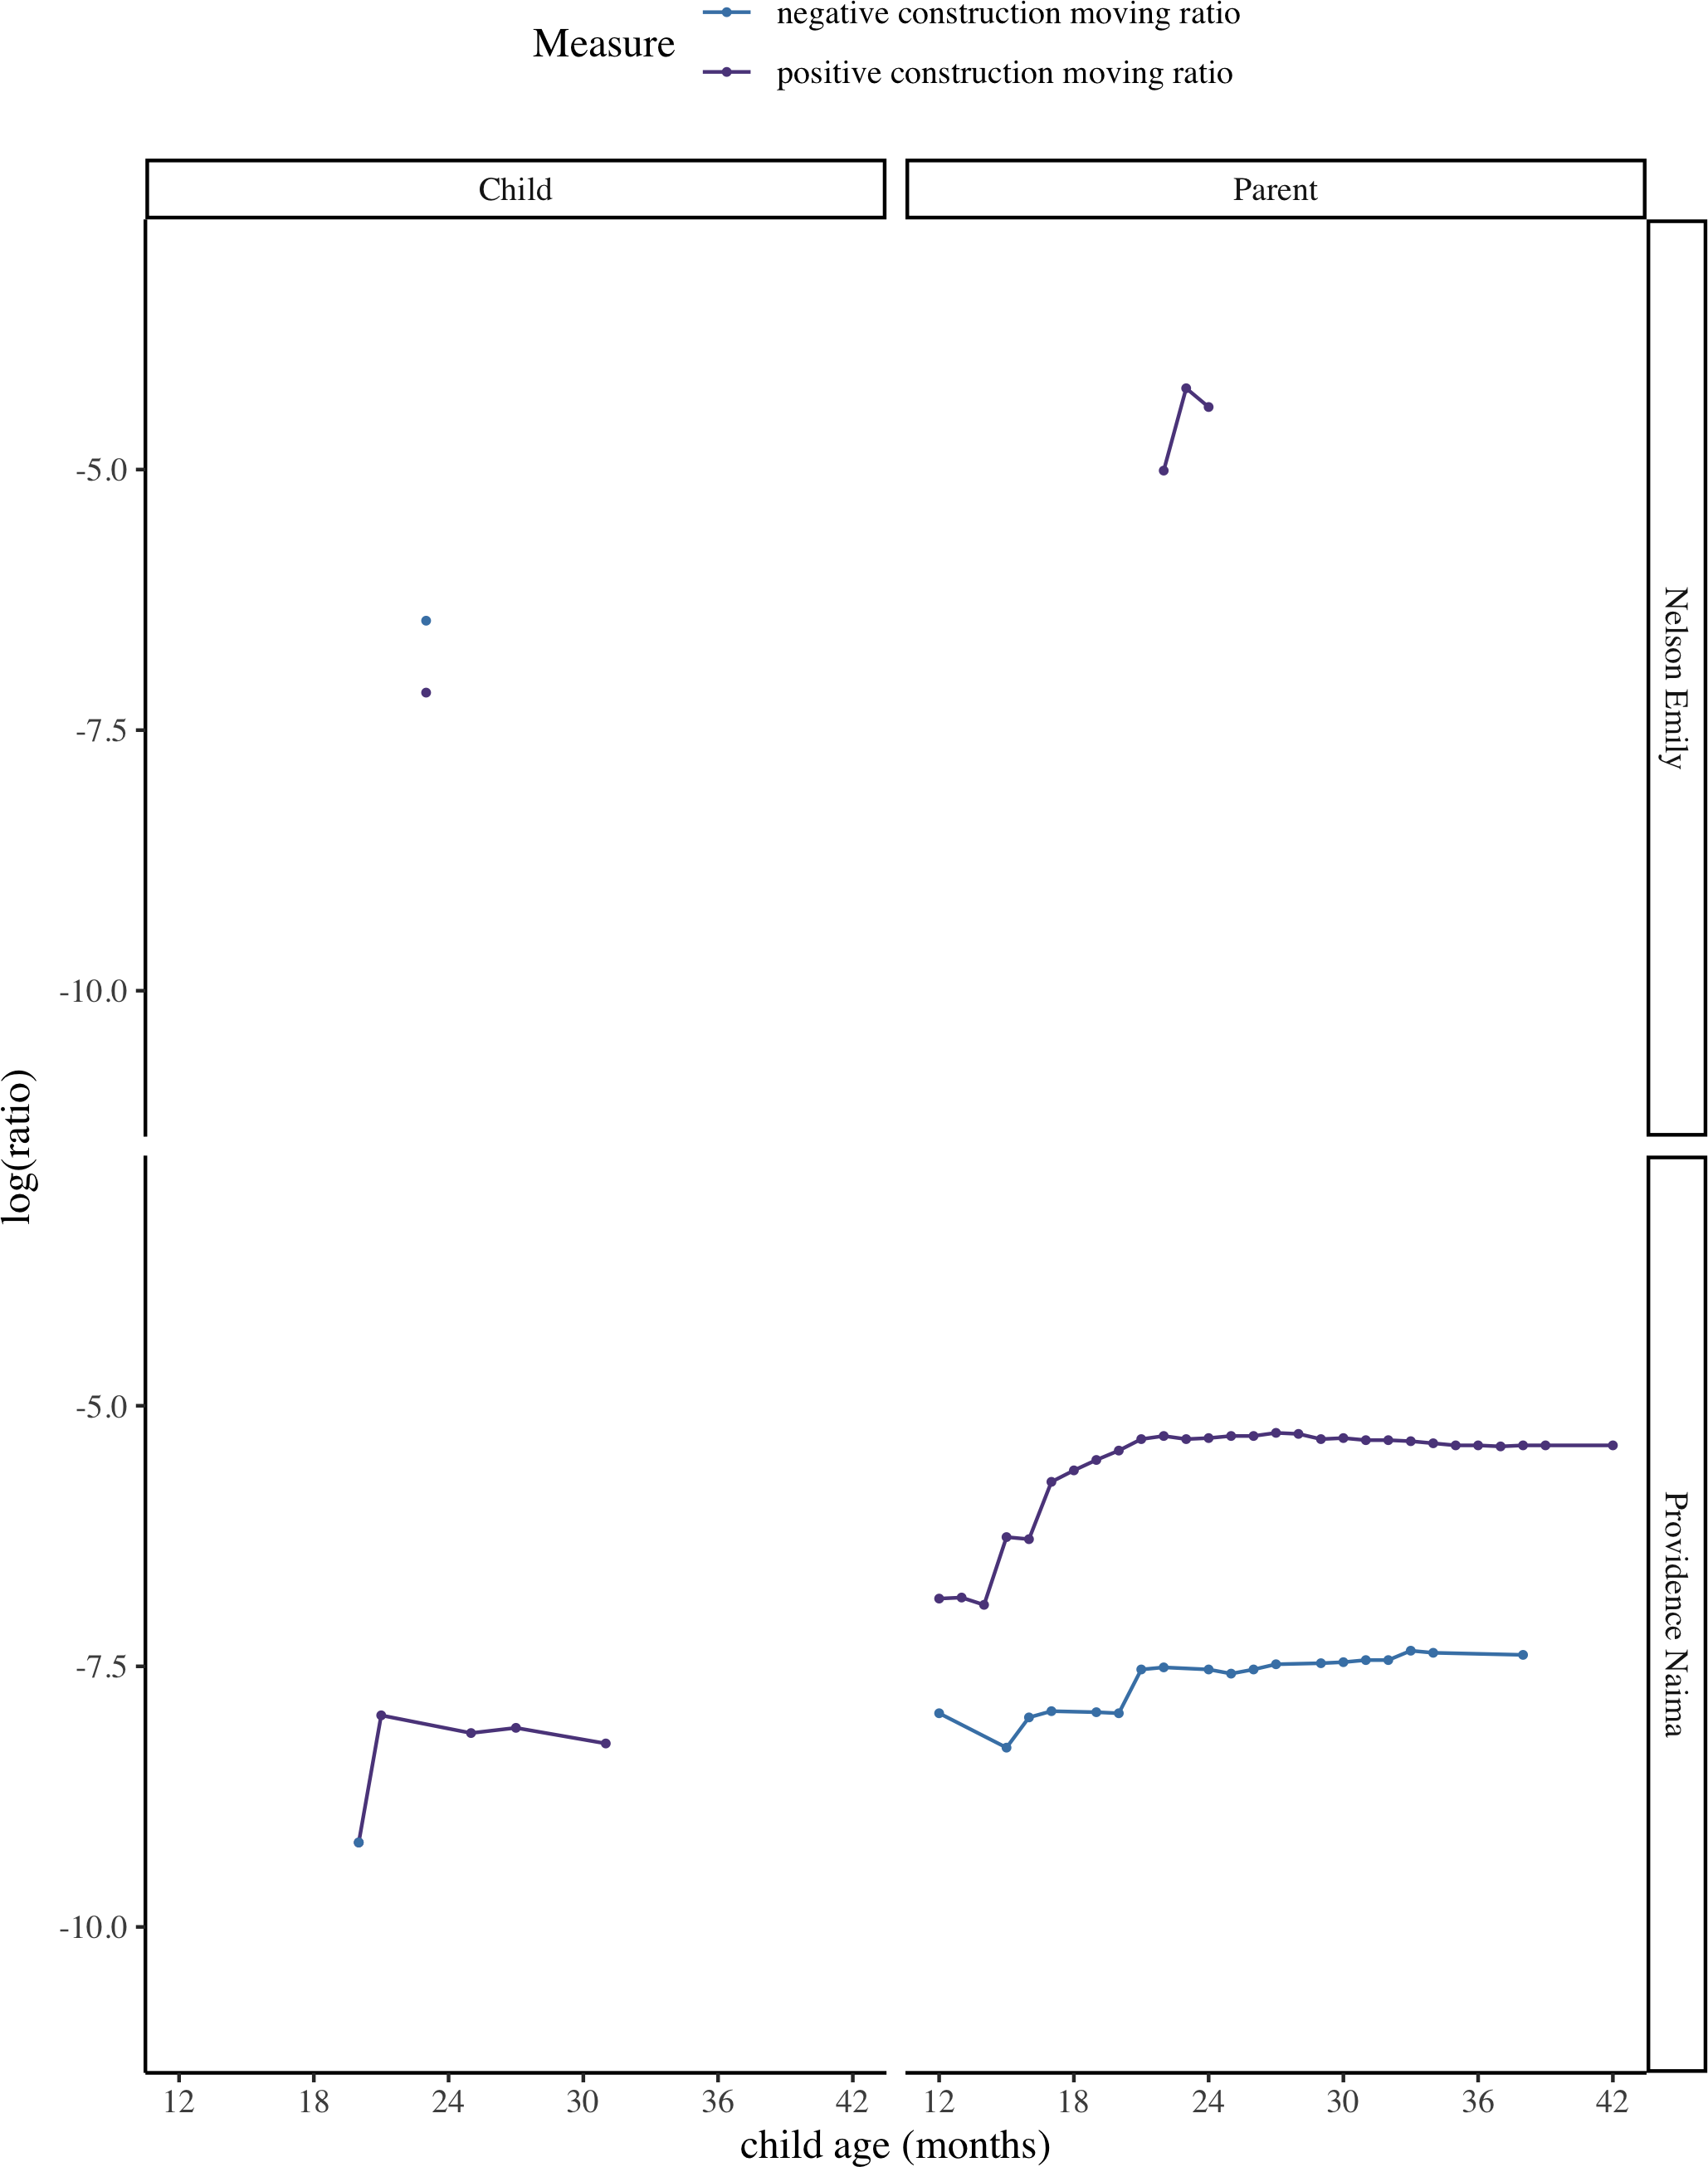
\includegraphics{neg_construction_article_files/figure-latex/individualepistemicremember-1} 

}

\caption{Individual variation for Epistemic negation and its positive counterparts, when the head verb is remember}\label{fig:individualepistemicremember}
\end{figure}

\begin{figure}[H]

{\centering 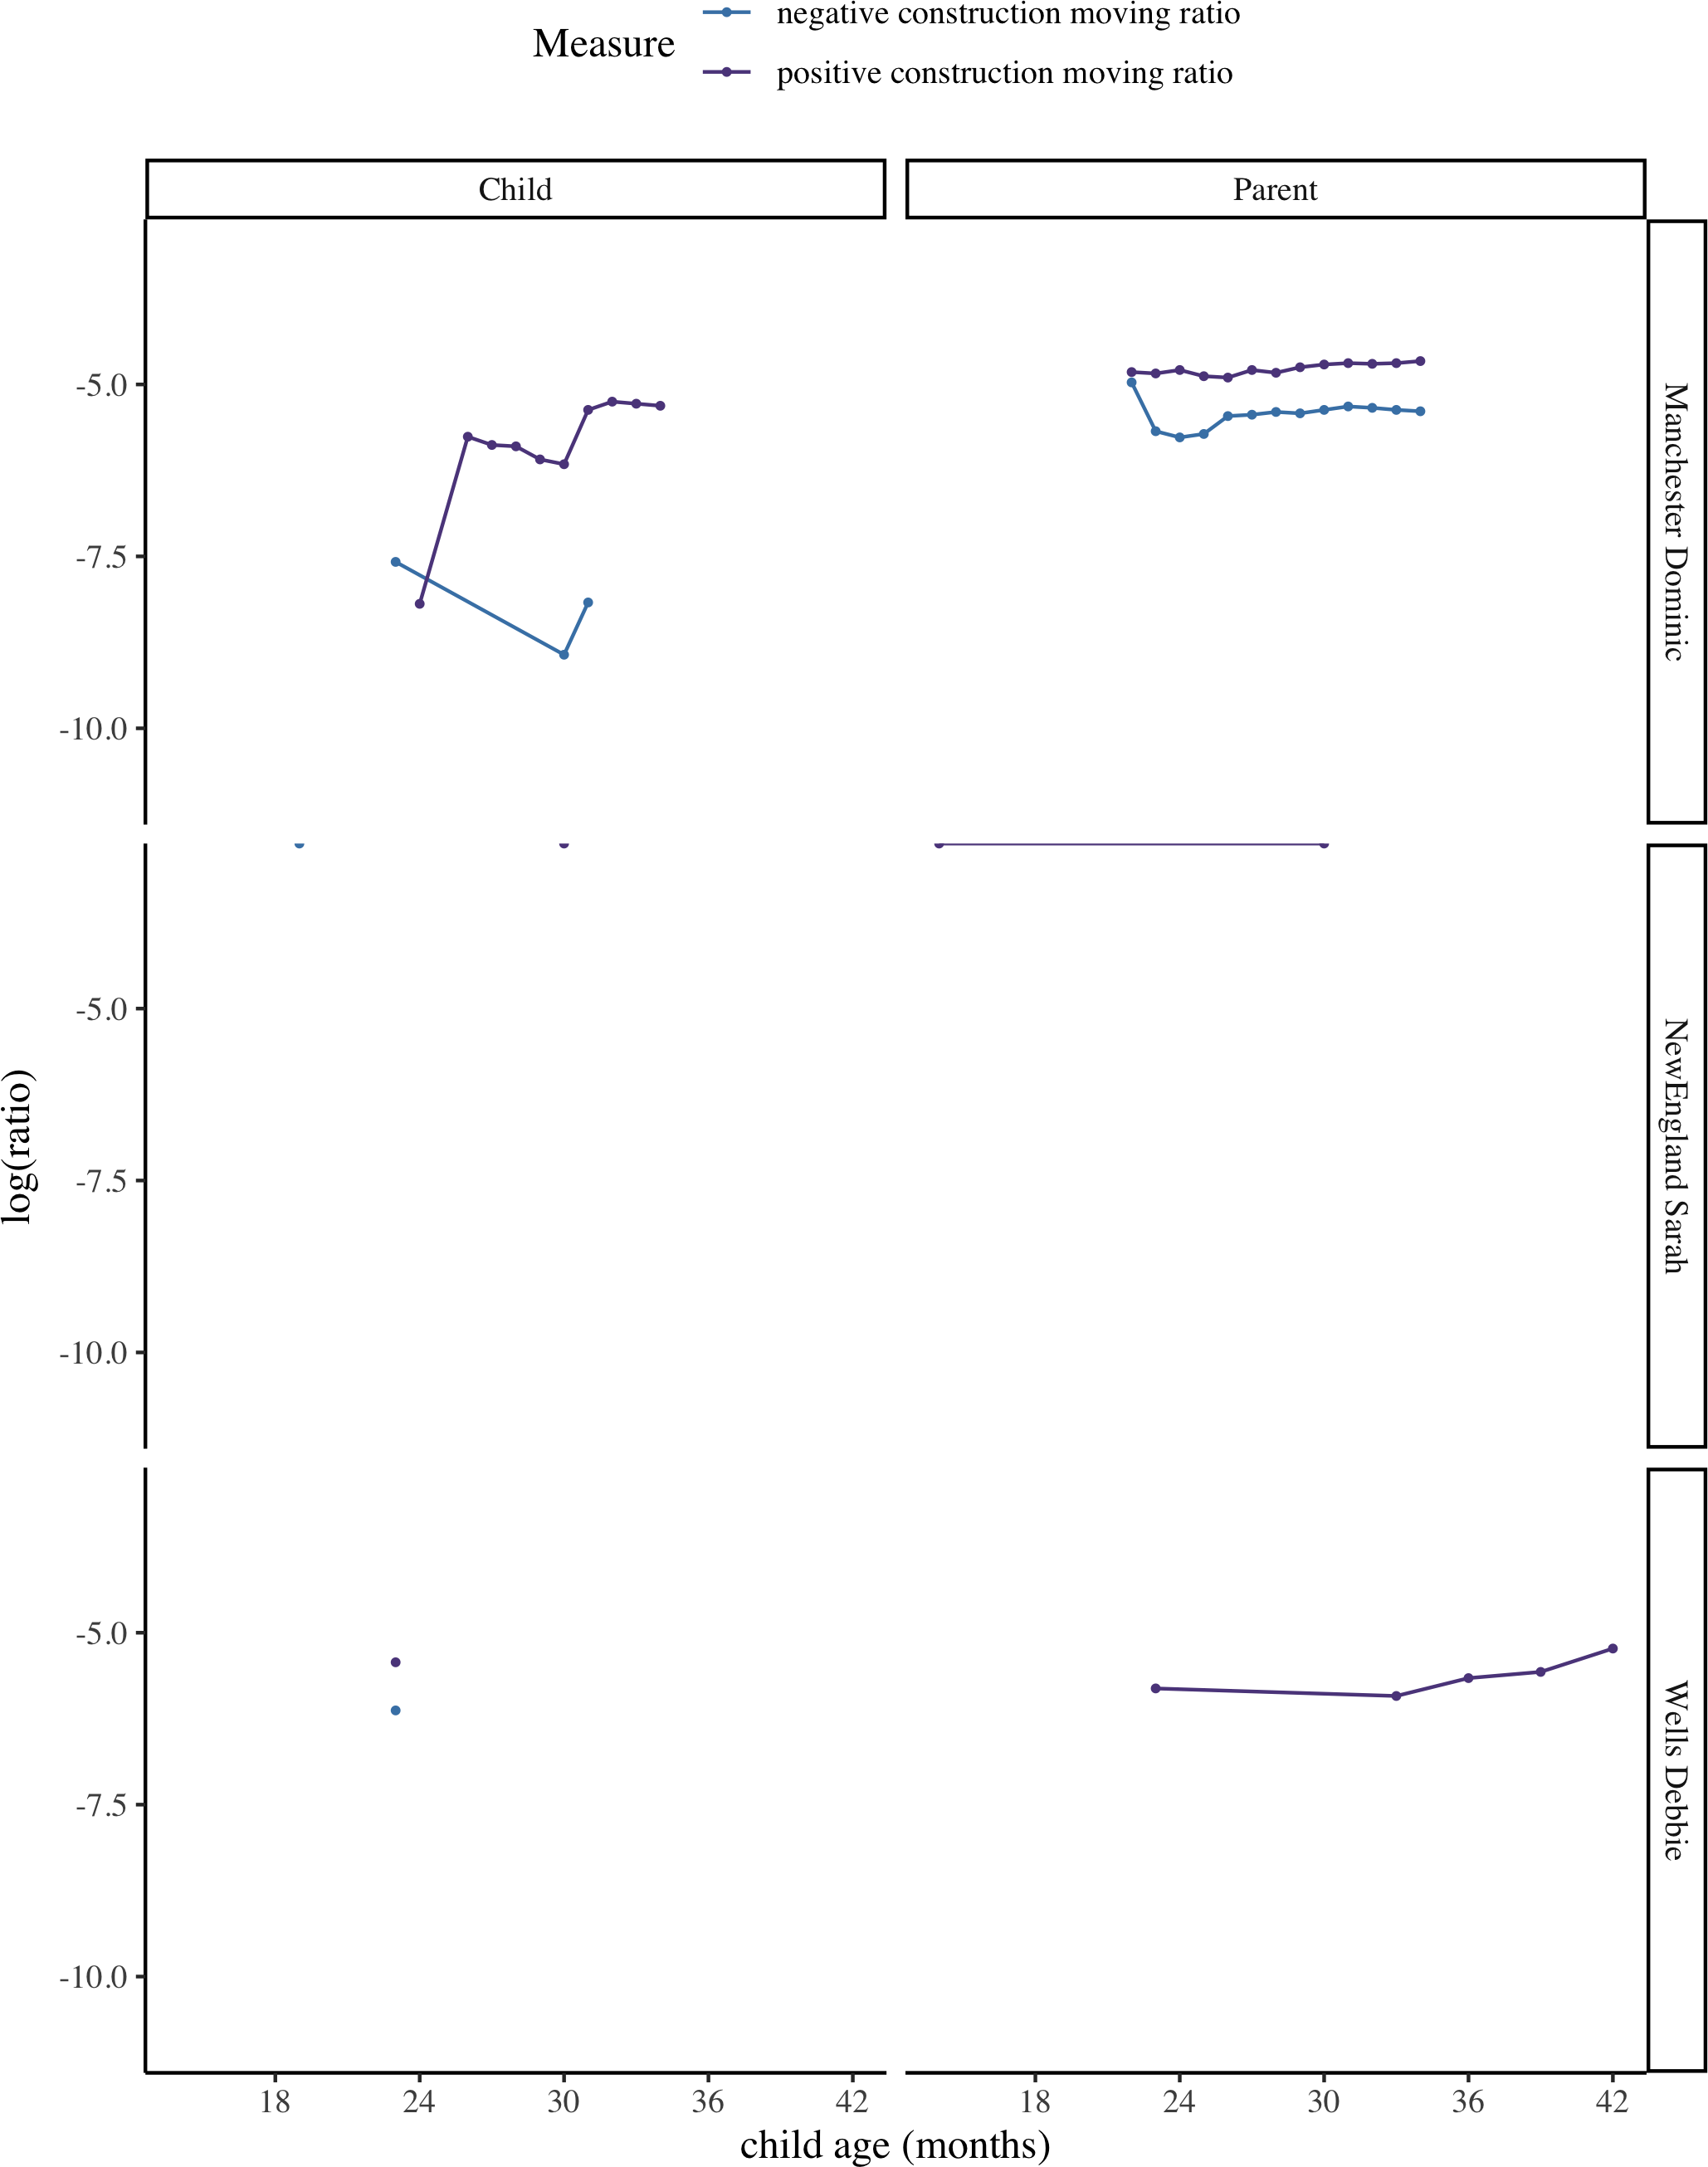
\includegraphics{neg_construction_article_files/figure-latex/individualepistemicthink-1} 

}

\caption{Individual variation for Epistemic negation and its positive counterparts, when the head verb is think}\label{fig:individualepistemicthink}
\end{figure}

\clearpage

\hypertarget{possession}{%
\subsubsection{Possession}\label{possession}}

The last function we explored is possession. We selected cases where the negative morphemes are combined with auxiliary verbs to modify a head verb with the lemma form \emph{have} (e.g.~(15)). We also included individual noun phrases with possessive pronouns as heads and modified by negative morphemes (e.g.~(16)). Cases in which the syntactic head of the negative morphemes is a predicate of a copula verb (e.g.~\enquote{this is not mine}) were excluded to separate them from the function \enquote{labeling}. The number of negative utterances that were subjected to analysis for this function is 66,783 (child: 19,097; parent: 47,686).

~
(15) \emph{I don't have it}

~
(16) \emph{not mine}

Given Figure 7, the developmental trajectory for possession in child speech appears to have notable differences depending on what the negative morphemes are modifying. When their syntactic head is \emph{have}, the pattern is comparable to those of \enquote{rejection} and \enquote{labeling}, where children are increasing their combination of negative morphemes from 18 to 36 months. However, the production moving ratio for utterances headed by possessive pronouns seems to be relatively stable across different ages.

\begin{figure}[H]

{\centering 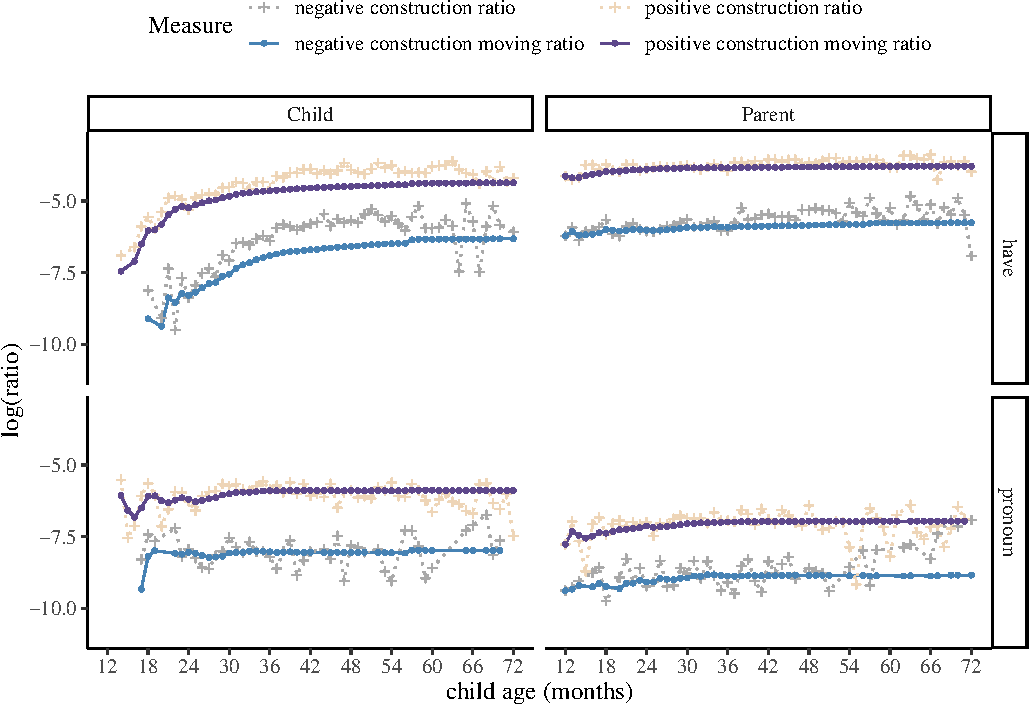
\includegraphics{neg_construction_article_files/figure-latex/possession-1} 

}

\caption{Possession and its positive counterparts}\label{fig:possession}
\end{figure}

\begin{figure}[H]

{\centering 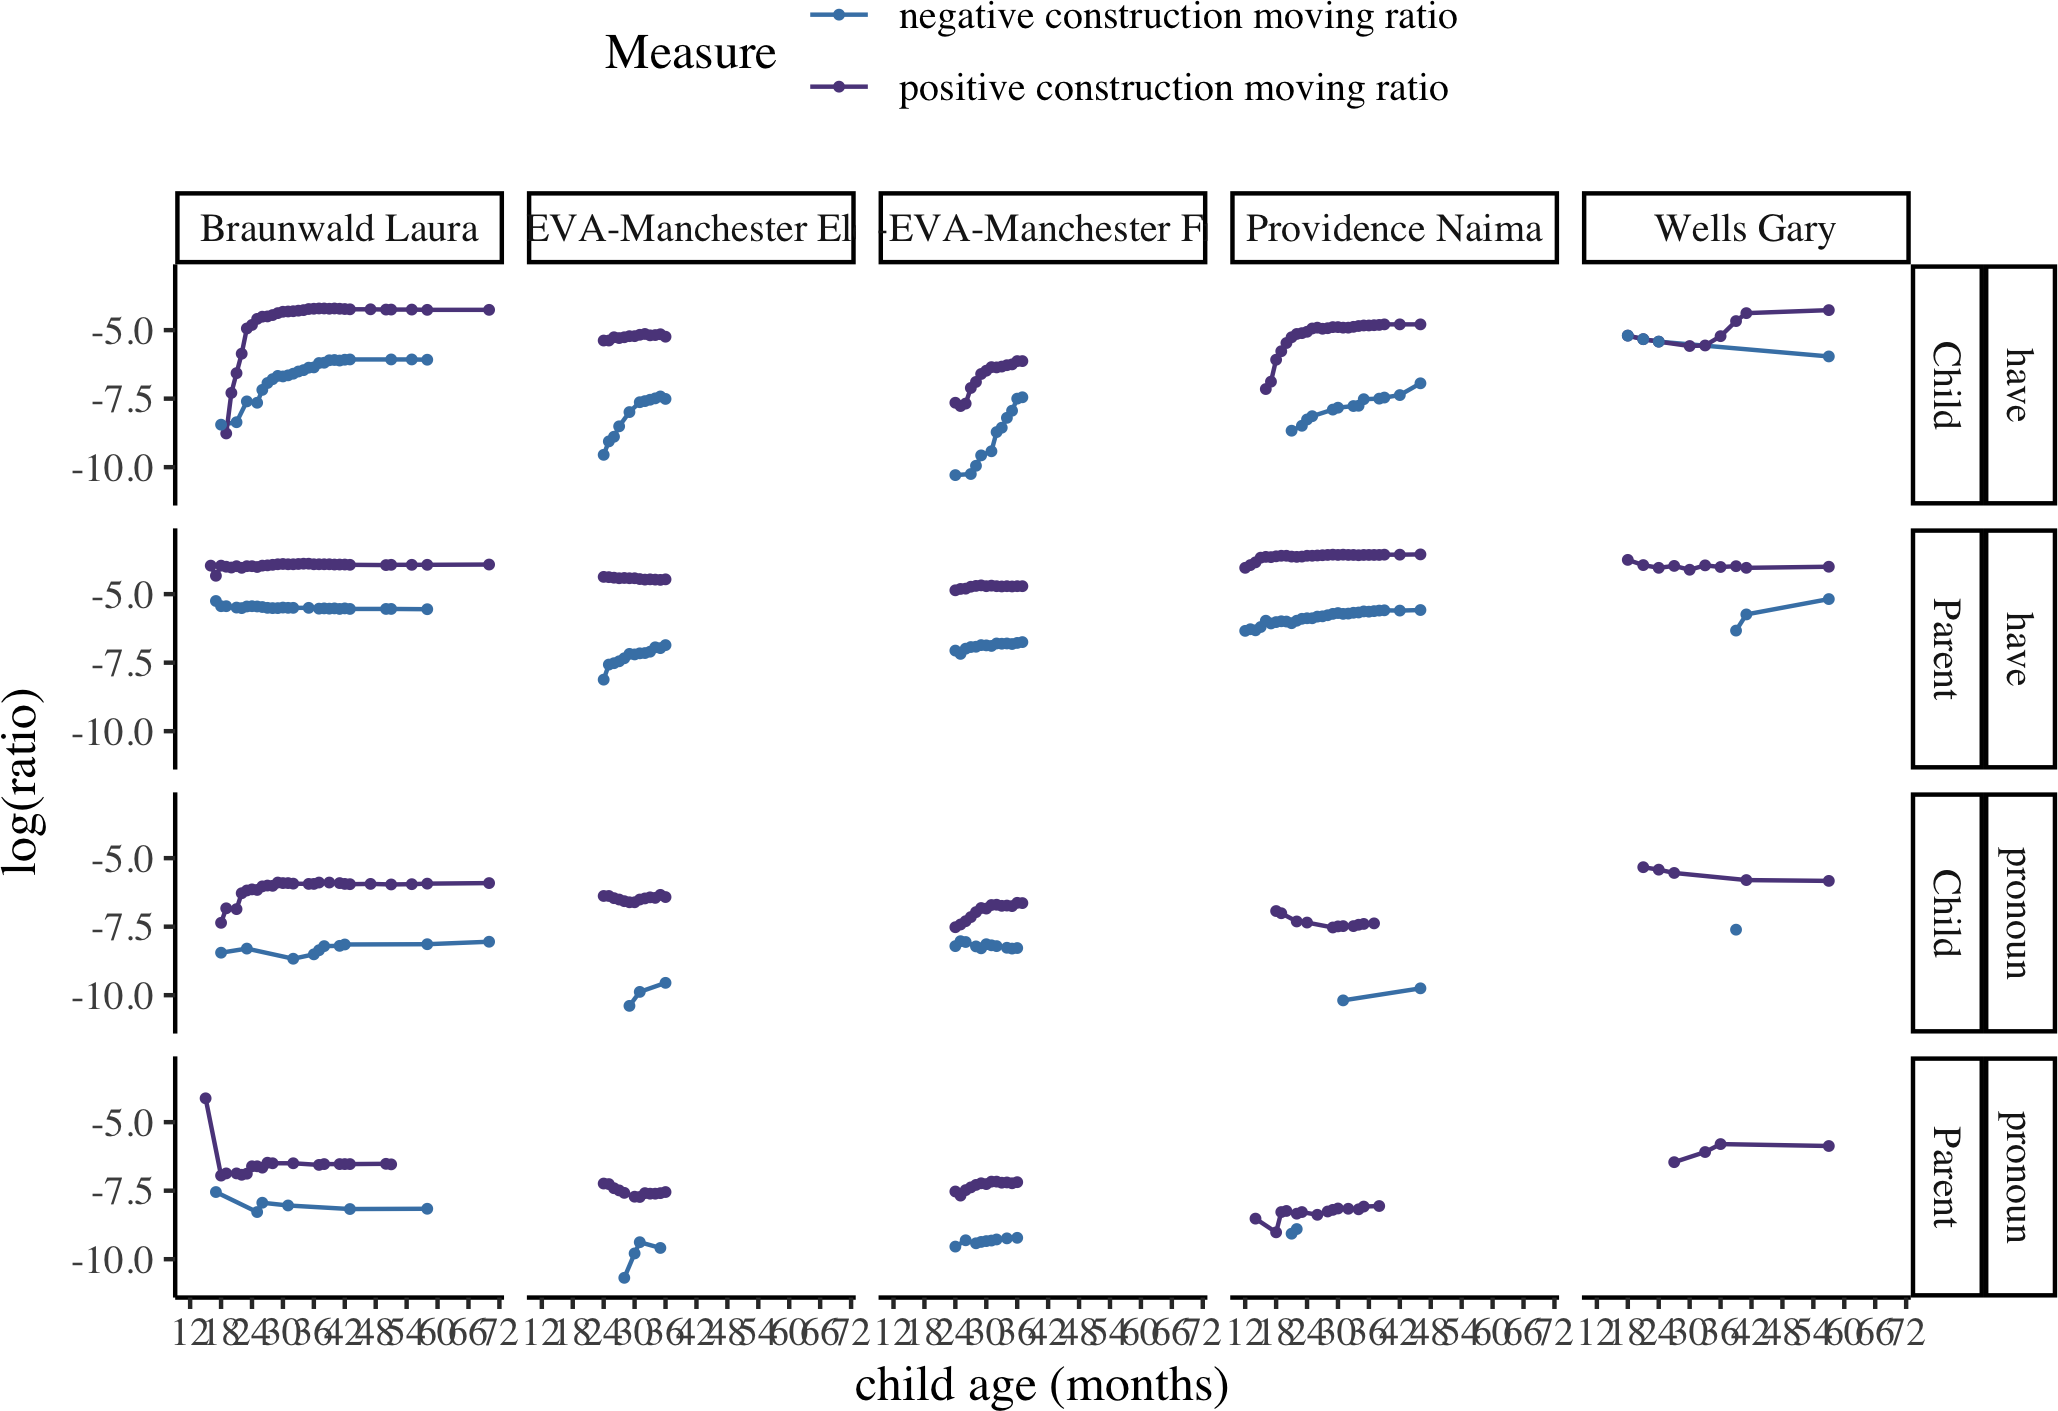
\includegraphics{neg_construction_article_files/figure-latex/individualpossession-1} 

}

\caption{Individual variation for Possession and its positive counterparts}\label{fig:individualpossession}
\end{figure}

\begin{figure}[H]

{\centering 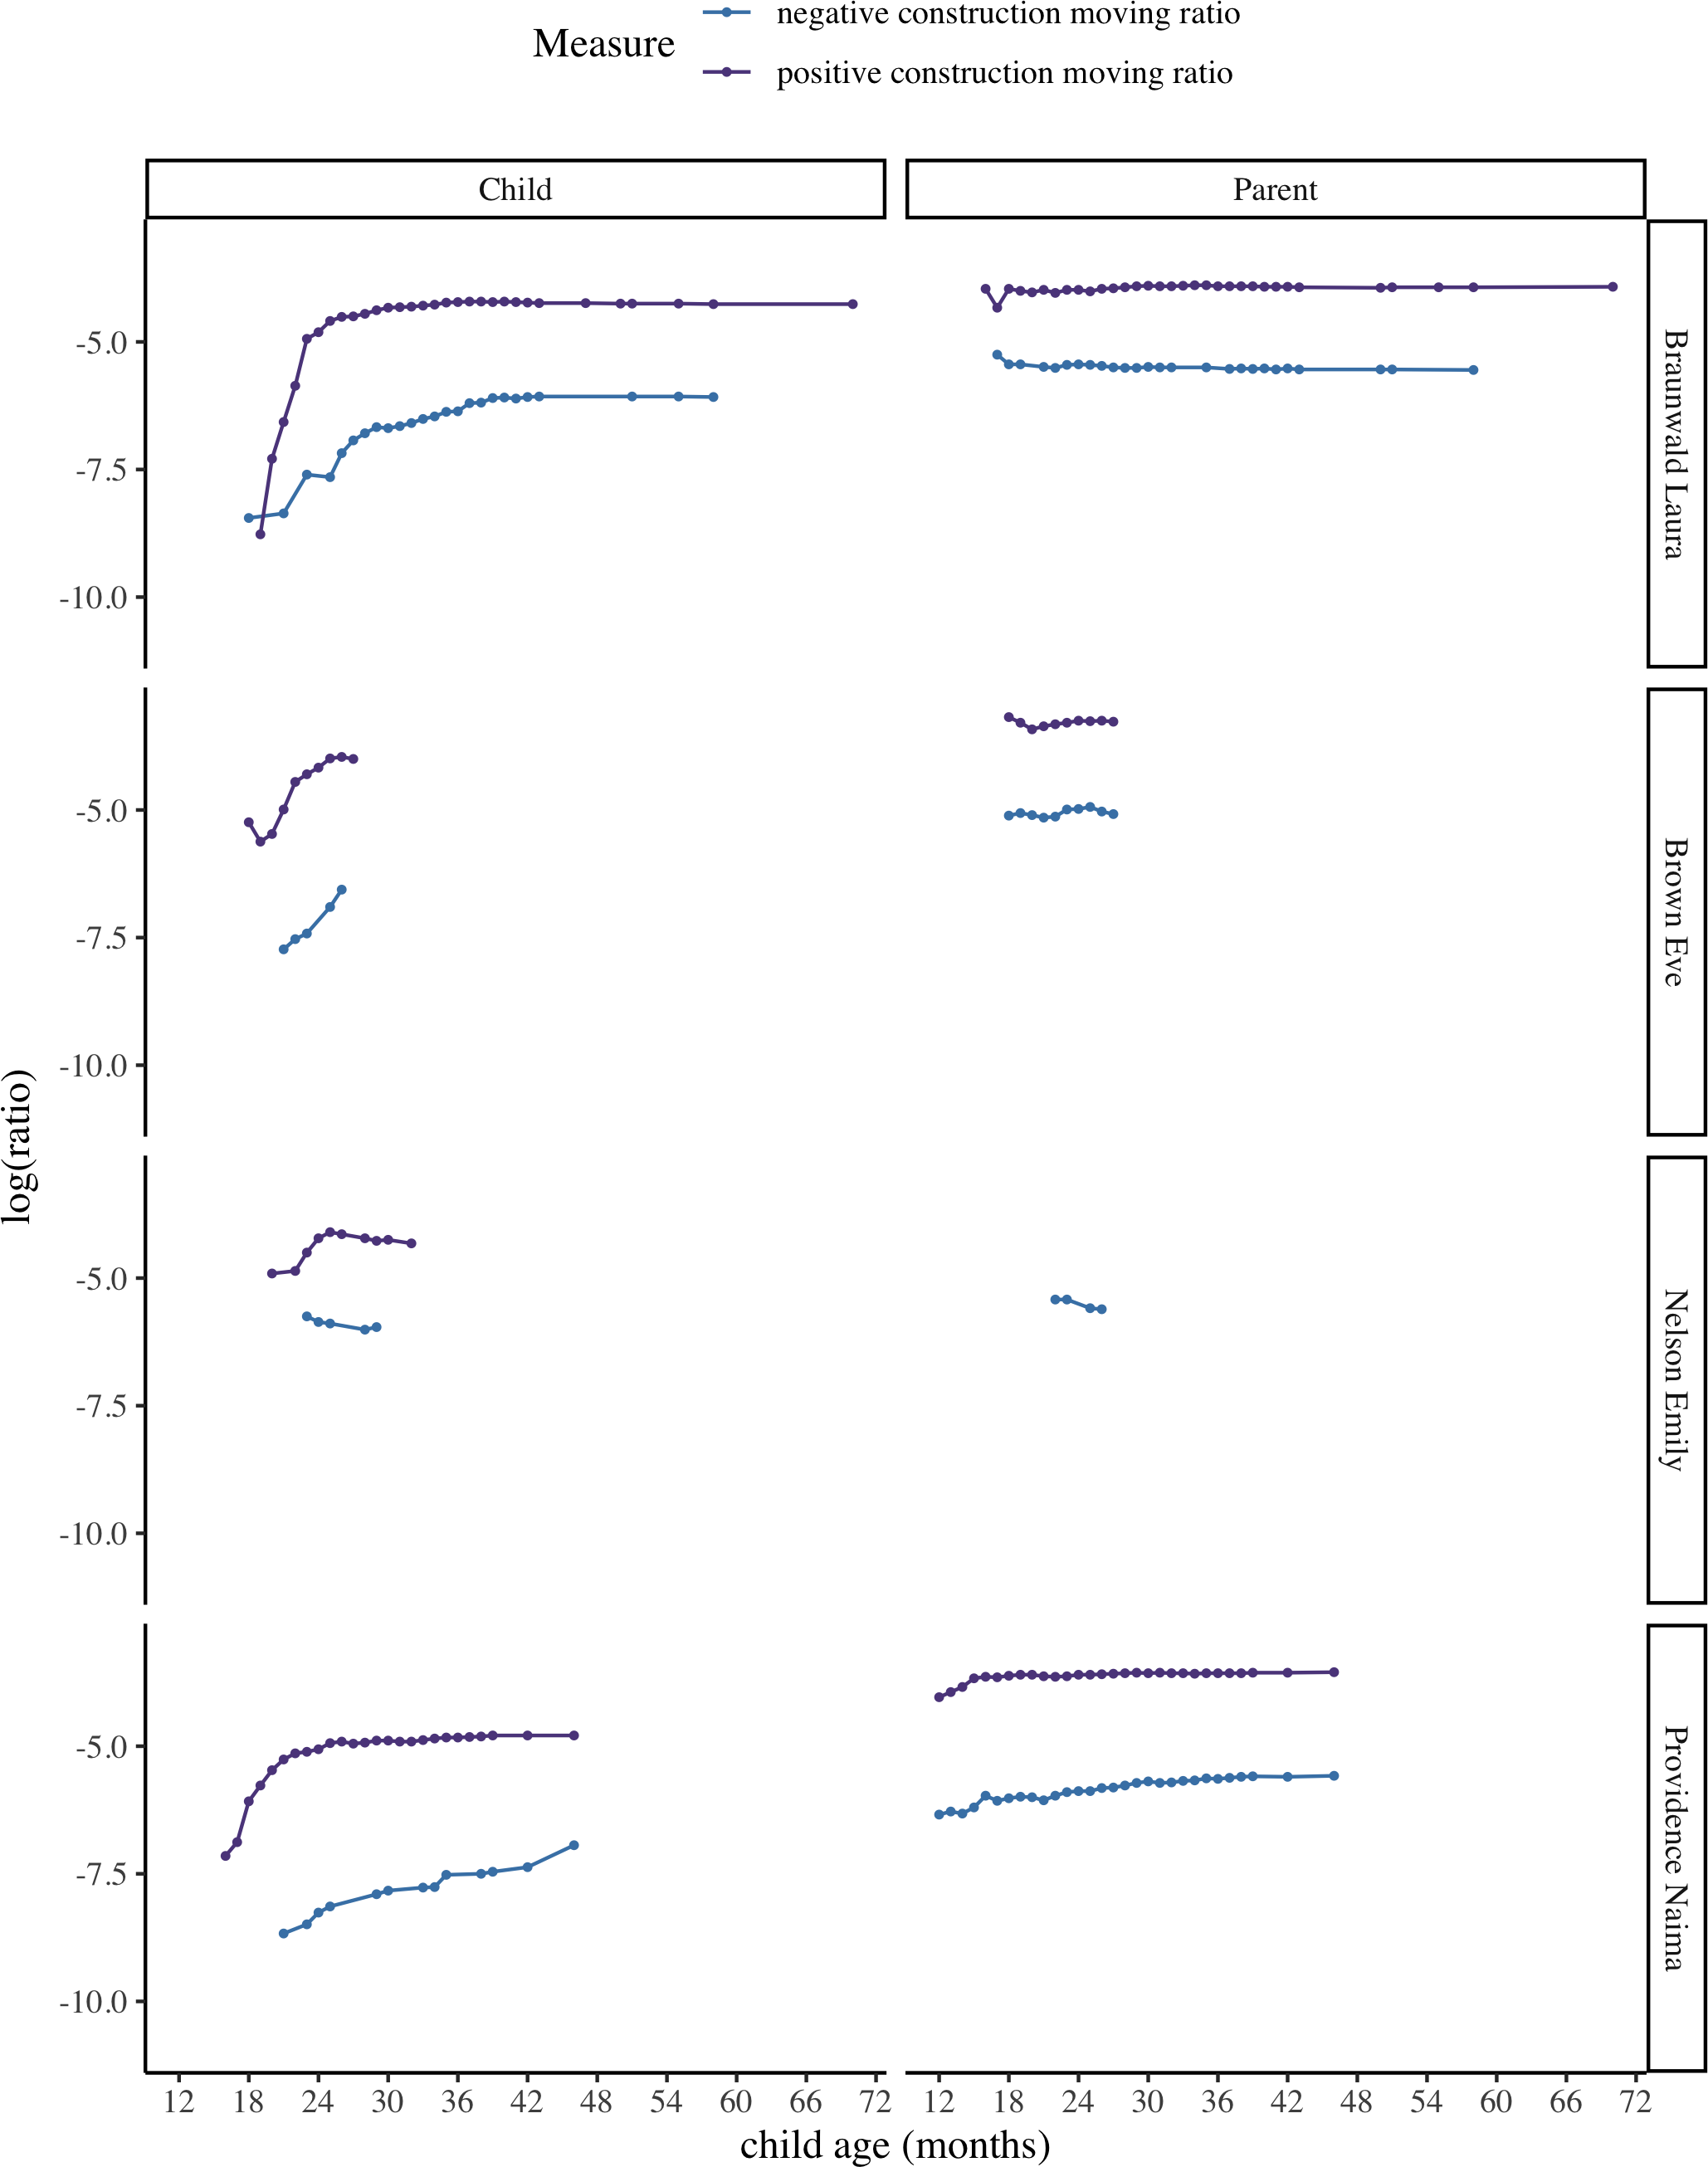
\includegraphics{neg_construction_article_files/figure-latex/individualpossessionhave-1} 

}

\caption{Individual variation for Possession and its positive counterparts, when the head verb is have}\label{fig:individualpossessionhave}
\end{figure}

\begin{figure}[H]

{\centering 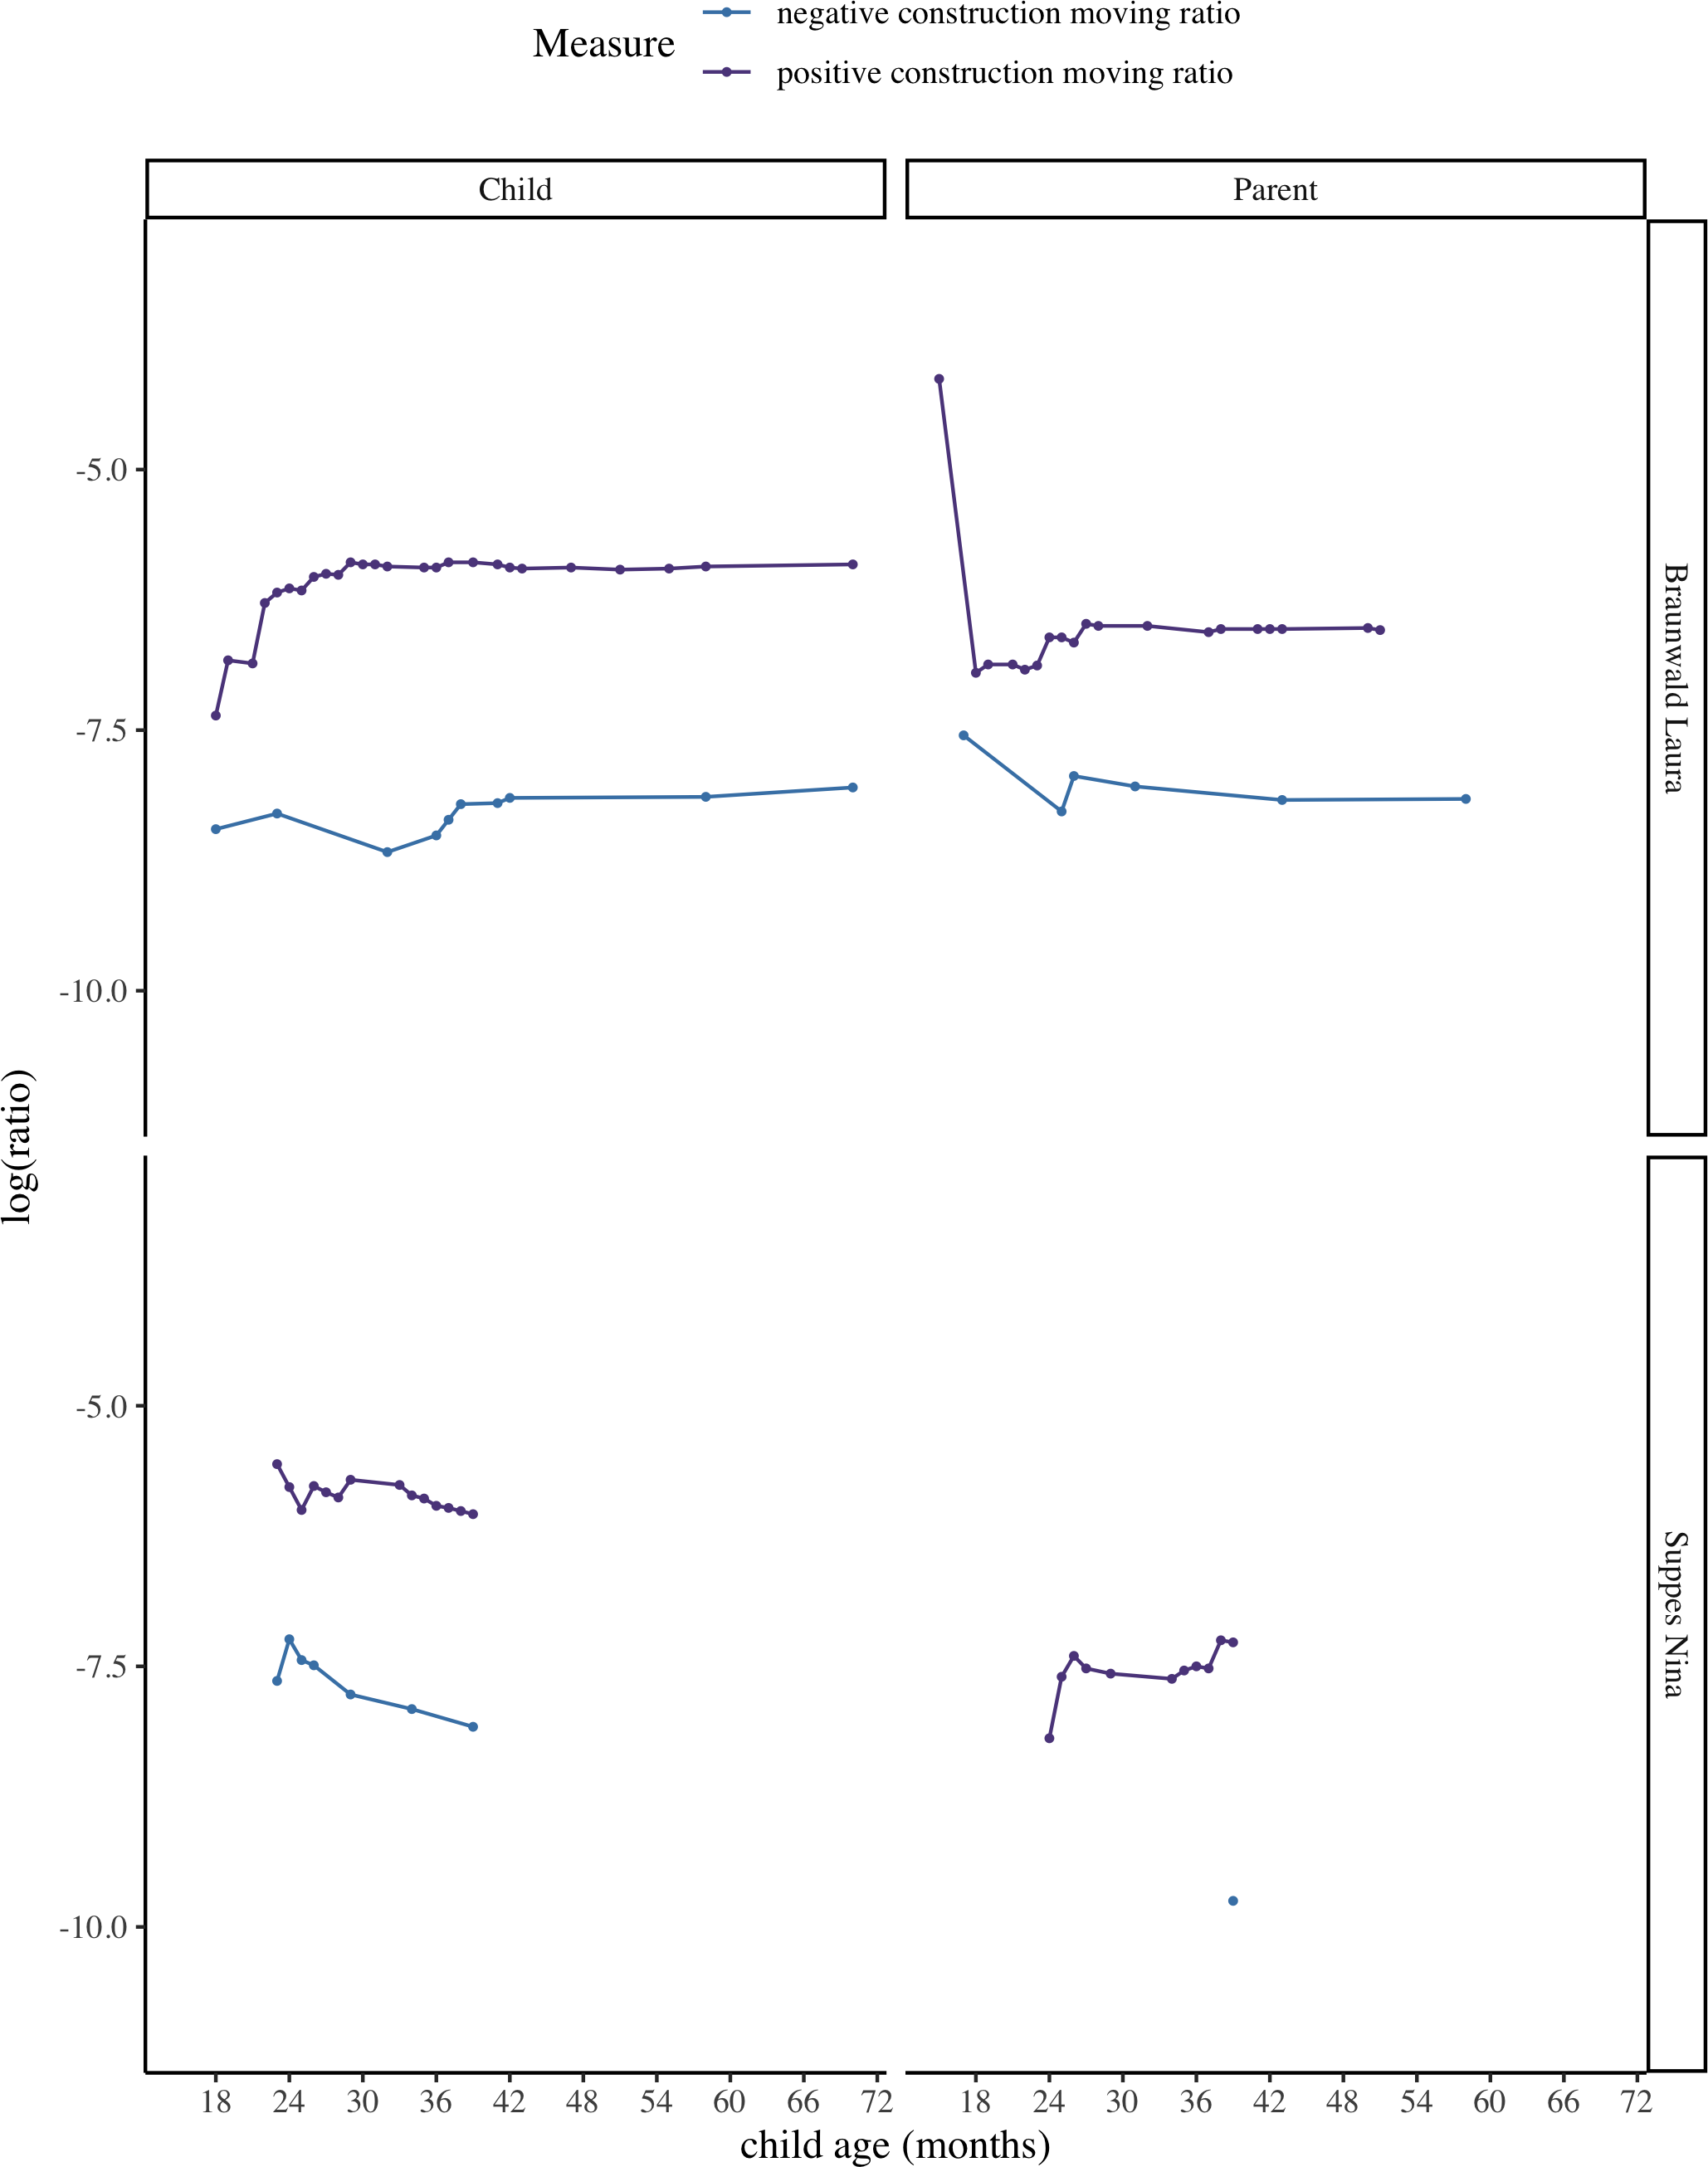
\includegraphics{neg_construction_article_files/figure-latex/individualpossessionpro-1} 

}

\caption{Individual variation for Possession and its positive counterparts, when the syntactic head is a pronoun}\label{fig:individualpossessionpro}
\end{figure}

\clearpage

\hypertarget{an-overall-look}{%
\subsubsection{An overall look}\label{an-overall-look}}

\begin{figure}[H]

{\centering 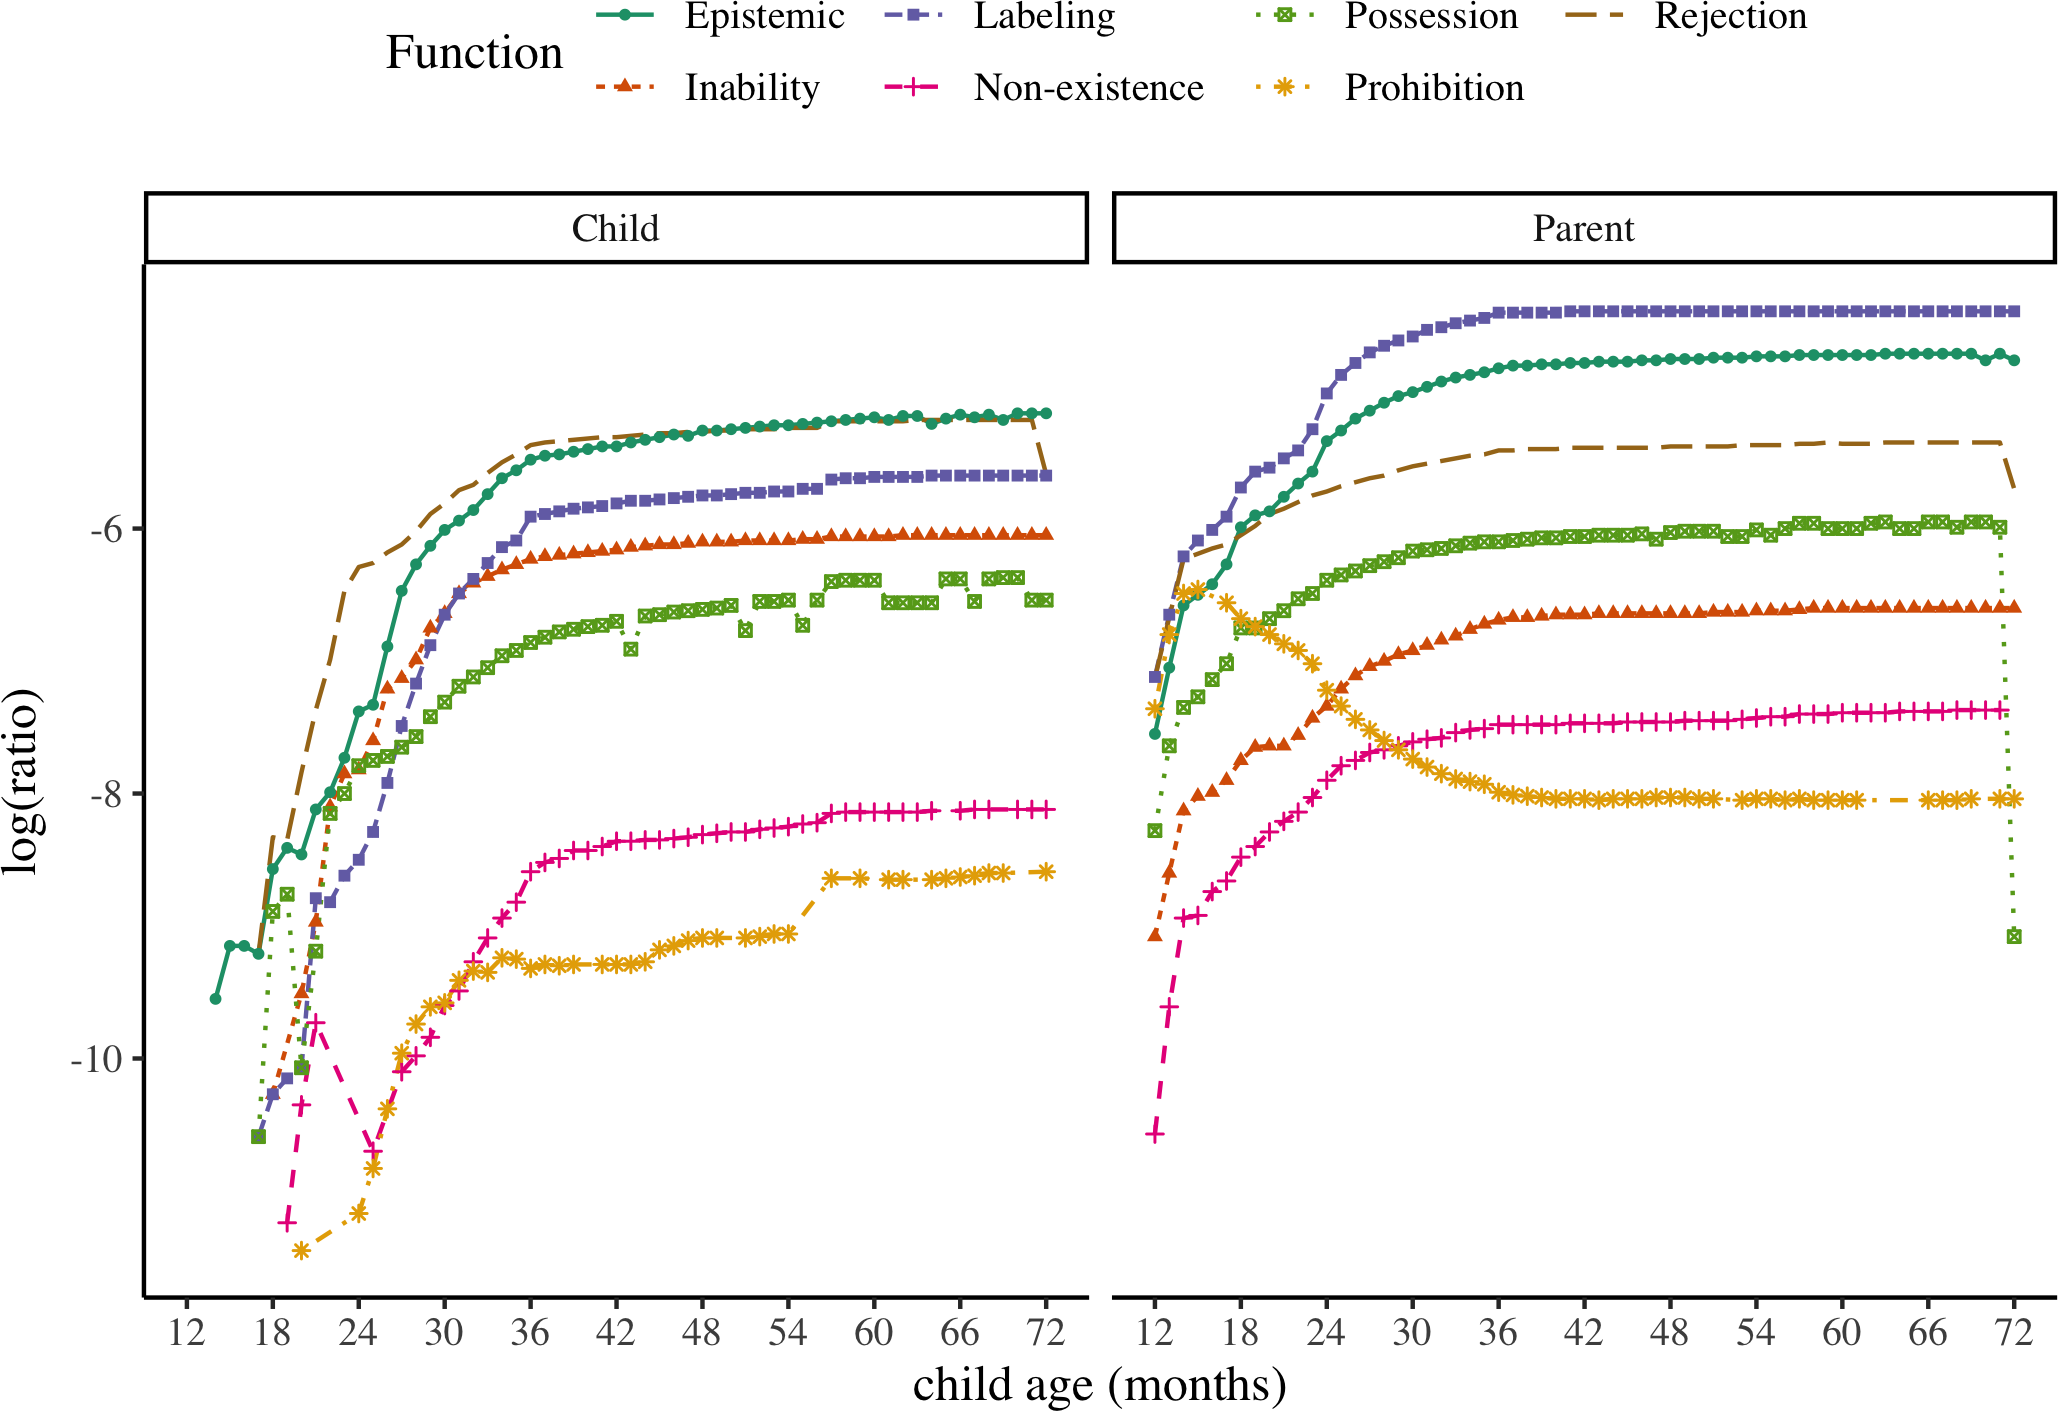
\includegraphics{neg_construction_article_files/figure-latex/allneg-1} 

}

\caption{All negative functions}\label{fig:allneg}
\end{figure}

\clearpage

\begin{figure}[H]

{\centering 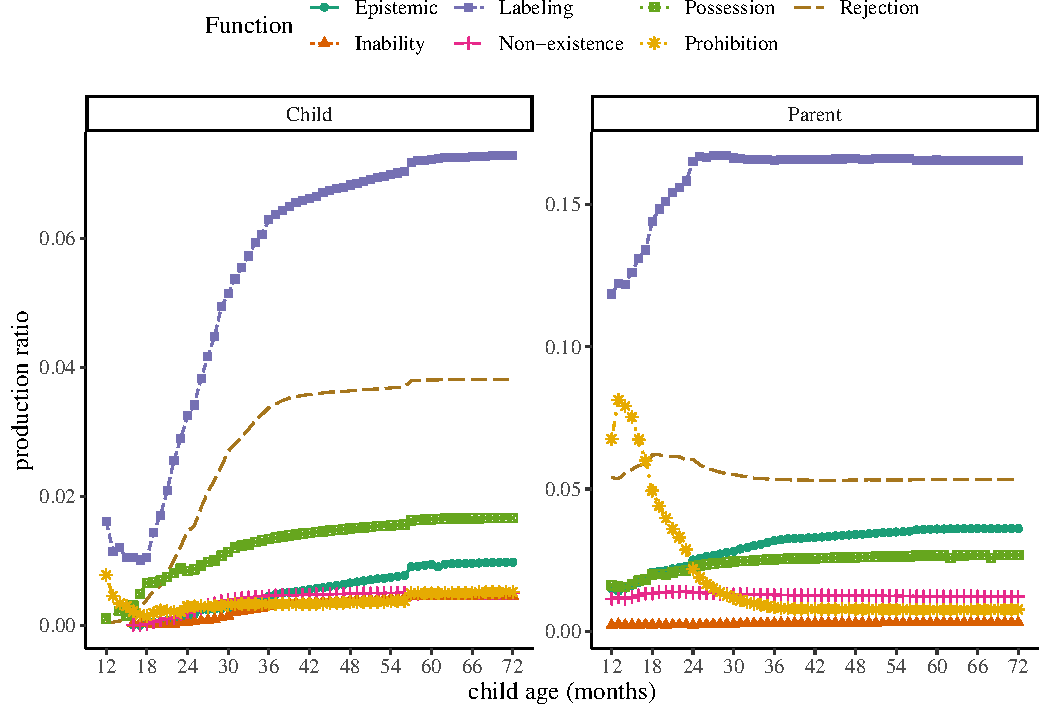
\includegraphics{neg_construction_article_files/figure-latex/allpos-1} 

}

\caption{Positive counpterparts of all negative functions}\label{fig:allpos}
\end{figure}

\hypertarget{discussion}{%
\section{Discussion}\label{discussion}}

Using automatic annotations of large-scale corpora of child-parent interactions, we presented production trajectories for seven negative constructions that tend to express rejection, non-existence, prohibition, inability, labeling, epistemic states, and possession (Table 1). The results suggest that the production of almost all these negative constructions (except for prohibition) emerges and gradually increases within the 18-36 months age range (Figure 8). Their production frequencies remain stable and regular after 36 months and relatively close to parents' levels of production. It is important to note that similar to prior studies, our conclusions are limited to negation in children's production. Systematic experiments testing children's comprehension of negative utterances with different communicative functions are necessary to better understand the origins and developmental trajectory of negation.

For future work, we would like to explore several directions. First, to more thoroughly examine and potentially model the developmental trajectories of negation in child production, certain production-specific factors (e.g.~length of utterance, ease of pronunciation) should be taken into account as well. In addition, we aim to investigate the production trajectory of positive counterparts to our negative structures (e.g.~\enquote{I know} for \enquote{I don't know}). Comparisons of negative utterances in relation to their positive counterparts would allow us to further analyze the developmental paths of negation within specific constructions.

Lastly, our experiments have concentrated on larger syntactic structures at the utterance level, hence cases where negation is used as discourse markers to respond to previous utterance(s) were excluded. However, these instances also have important semantic and conceptual roles in the communication between children and parents (e.g.~parent: \emph{do you want some bread?}; child: \emph{no no no}). Thus inclusions of negative structures at a more comprehensive level would be able to paint a more clear picture about the development of negation.

\begingroup
\setlength{\parindent}{-0.5in}
\setlength{\leftskip}{0.5in}

\endgroup

\hypertarget{refs}{}
\leavevmode\hypertarget{ref-diaparser}{}%
Attardi, G., Sartiano, D., \& Yu, Z. (n.d.). DiaParser attentive dependency parser. \emph{Submitted for Publication}.

\leavevmode\hypertarget{ref-bloom1970language}{}%
Bloom, L. M. (1970). \emph{Language development: Form and function in emerging grammars} (PhD thesis). Columbia University.

\leavevmode\hypertarget{ref-cameron2007part}{}%
Cameron-Faulkner, T., Lieven, E., \& Theakston, A. (2007). What part of no do children not understand? A usage-based account of multiword negation. \emph{Journal of Child Language}, \emph{34}(2), 251.

\leavevmode\hypertarget{ref-choi1988semantic}{}%
Choi, S. (1988). The semantic development of negation: A cross-linguistic longitudinal study. \emph{Journal of Child Language}, \emph{15}(3), 517--531.

\leavevmode\hypertarget{ref-clark2010adult}{}%
Clark, E. V. (2010). Adult offer, word-class, and child uptake in early lexical acquisition. \emph{First Language}, \emph{30}(3-4), 250--269.

\leavevmode\hypertarget{ref-darwin1872expression}{}%
Darwin, C. (1872). \emph{The expression of the emotions in man and animals}. John Murray.

\leavevmode\hypertarget{ref-demuth2006word}{}%
Demuth, K., Culbertson, J., \& Alter, J. (2006). Word-minimality, epenthesis and coda licensing in the early acquisition of English. \emph{Language and Speech}, \emph{49}(2), 137--173.

\leavevmode\hypertarget{ref-macwhinney2000childes}{}%
MacWhinney, B. (2000). \emph{The childes project: Tools for analyzing talk. Transcription format and programs} (Vol. 1). Psychology Press.

\leavevmode\hypertarget{ref-nordmeyer2018individual}{}%
Nordmeyer, A., \& Frank, M. C. (2018). Individual variation in children's early production of negation. \emph{Proceedings of the 40th annual meeting of the cognitive science society}, 2167--2172.

\leavevmode\hypertarget{ref-pea1978}{}%
Pea, R. (1978). \emph{The development of negation in early child language} (PhD thesis). University of Oxford.

\leavevmode\hypertarget{ref-sagae2010morphosyntactic}{}%
Sagae, K., Davis, E., Lavie, A., MacWhinney, B., \& Wintner, S. (2010). Morphosyntactic annotation of childes transcripts. \emph{Journal of Child Language}, \emph{37}(3), 705--729.

\leavevmode\hypertarget{ref-sanchez2019childes}{}%
Sanchez, A., Meylan, S. C., Braginsky, M., MacDonald, K. E., Yurovsky, D., \& Frank, M. C. (2019). Childes-db: A flexible and reproducible interface to the child language data exchange system. \emph{Behavior Research Methods}, \emph{51}(4), 1928--1941.

\leavevmode\hypertarget{ref-dg}{}%
Tesnière, L. (1959). \emph{Éléments de syntaxe structurale}. Paris: Klincksieck.

\leavevmode\hypertarget{ref-de1979form}{}%
Villiers, P. A. de, \& Villiers, J. G. de. (1979). Form and function in the development of sentence negation. \emph{Papers and Reports on Child Language Development}, \emph{17}, 57--64.

\leavevmode\hypertarget{ref-wei2006time}{}%
Wei, W. W. (2006). Time series analysis. In \emph{The oxford handbook of quantitative methods in psychology: Vol. 2}.


\end{document}
